%% This is the ctufit-thesis example file. It is used to produce theses
%% for submission to Czech Technical University, Faculty of Information Technology.
%%
%% This is version 1.6.3, built 16. 3. 2026.
%% 
%% Get the newest version from
%% https://gitlab.fit.cvut.cz/theses-templates/FITthesis-LaTeX
%%
%%
%% Copyright 2024, Tomas Novacek
%% Copyright 2021, Eliska Sestakova and Ondrej Guth
%%
%% This work may be distributed and/or modified under the
%% conditions of the LaTeX Project Public License, either version 1.3
%% of this license or (at your option) any later version.
%% The latest version of this license is in
%%  https://www.latex-project.org/lppl.txt
%% and version 1.3 or later is part of all distributions of LaTeX
%% version 2005/12/01 or later.
%%
%% This work has the LPPL maintenance status `maintained'.
%%
%% The current maintainer of this work is Tomas Novacek (novacto3@fit.cvut.cz).
%% Alternatively, submit bug reports to the tracker at
%% https://gitlab.fit.cvut.cz/theses-templates/FITthesis-LaTeX/issues
%%
%%

% arara: xelatex
% arara: biber
% arara: xelatex
% arara: xelatex

%%%%%%%%%%%%%%%%%%%%%%%%%%%%%%%%%%%%%%%%%
% CLASS OPTIONS
% language: czech/english/slovak
% thesis type: bachelor/master/dissertation/doctoral-report
% electronic (oneside) or printed (twoside), twoside is default
% paragraph - if passed, this optional argument sets paragraphs as the deepest level of headers, styles it, numbers it and adds it to Table of Content. Use with care! Normally, it is considered unwise to use it, since it is too deep.
% colour: bw for black&white OR no option for default colour scheme
%%%%%%%%%%%%%%%%%%%%%%%%%%%%%%%%%%%%%%%%%
\documentclass[english,bachelor,unicode,oneside]{ctufit-thesis}

%%%%%%%%%%%%%%%%%%%%%%%%%%%%%%%%%%
% FILL IN THIS INFORMATION
%%%%%%%%%%%%%%%%%%%%%%%%%%%%%%%%%%
\ctufittitle{StudySpace: A Collaborative Web Application for Academic
Students} % replace with the title of your thesis
\ctufitauthorfull{Thet Oo Aung} % replace with your full name (first name(s) and then family name(s) / surname(s)) including academic degrees
\ctufitauthorsurnames{Aung} 
\ctufitauthorgivennames{Thet Oo} 
\ctufitsupervisor{Ing.\,Jan Blizničenko,\,Ph.D.}
\ctufitdepartment{Department of Software Engineering}
\ctufitprogram{Informatics} % replace with your study program
\ctufitspecialisation{Software Engineering} % replace with your specialisation
\ctufityear{2026} % replace with the year of your defence
\ctufitdeclarationplace{Prague} % replace with the place where you sign the declaration
\ctufitdeclarationdate{\today} % replace with the date of signature of the declaration
\ctufitabstractCZE{Tato bakalářská práce popisuje návrh a implementaci prototypu webové aplikace StudySpace, která umožňuje studentům a vyučujícím spravovat studijní materiály a spolupracovat v jednom prostředí. Aplikace řeší problém, kdy studenti dnes používají několik různých nástrojů najednou pro materiály, komunikaci i odevzdávání úkolů.

Práce zahrnuje analýzu existujících systémů pro správu výuki a následnou implementaci klíčových funkcí: správu kurzů, systém, ve kterém si student může naklonovat studijní pracovní prostor, přidat vlastní poznámky a upravený dokument přispět zpět na původní stránku kurzu ke kontrole vyučujícím, zasílání zpráv navázaných na konkrétní části obsahu a dotazování materiálů pomocí umělé inteligence. Backend je postaven na Java a Spring Boot, frontend na Next.js a React, databáze PostgreSQL a nasazení probíhá pomocí Dockeru. Systém je otestován jednotkovými, repozitářovými a integračními testy.}
\ctufitabstractENG{This bachelor's thesis describes the design and implementation of a prototype of StudySpace, a web application that allows students and instructors to manage course materials and collaborate in one place. The application addresses the problem of students having to switch between multiple separate tools for materials, communication, and assignments.

The thesis presents an analysis of existing learning management systems and system requirements, followed by the design and implementation of key features: course management, a system where students can clone a workspace, add their own notes, and contribute the updated document back to the original course page for the instructor to review, messages linked to specific parts of the content, and an AI assistant for querying study materials. The backend is built with Java and Spring Boot, the frontend with Next.js and React, using PostgreSQL for data storage and Docker for deployment. The system is verified with unit, repository, and integration tests.}
\ctufitkeywordsCZE{webová aplikace, spolupráce, React, Spring Boot, Next.js, PostgreSQL, REST API, Docker, WebSocket}
\ctufitkeywordsENG{web application, collaboration, React, Spring Boot, Next.js, PostgreSQL, REST API, Docker, WebSocket}
%%%%%%%%%%%%%%%%%%%%%%%%%%%%%%%%%%
% END FILL IN
%%%%%%%%%%%%%%%%%%%%%%%%%%%%%%%%%%

%%%%%%%%%%%%%%%%%%%%%%%%%%%%%%%%%%
% CUSTOMIZATION of this template
% Skip this part or alter it if you know what you are doing.
%%%%%%%%%%%%%%%%%%%%%%%%%%%%%%%%%%

\RequirePackage{iftex}[2020/03/06]
\iftutex % XeLaTeX and LuaLaTeX
    \RequirePackage{ellipsis}[2020/05/22] %ellipsis workaround for XeLaTeX
\else
    \errmessage{Only compilation with XeLaTeX or LuaLaTeX is allowed}
    \stop
\fi

% hyperlinks
\hypersetup{
    pdfpagelayout=TwoPageRight,
    colorlinks=false,
    allcolors=decoration,
    pdfborder={0 0 0.1}
}

% uncomment the following to hide all hyperlinks
%\hypersetup{hidelinks}

% uncomment the following to change the colour of all hyperlinks to CTU blue
%\hypersetup{allbordercolors=decoration}

\RequirePackage{pdfpages}[2020/01/28]

%%%%%%%%%%%%%%%%%%%%%%%%%%%%%%%%%%
% CUSTOMIZATION of this template END
%%%%%%%%%%%%%%%%%%%%%%%%%%%%%%%%%%


%%%%%%%%%%%%%%%%%%%%%%
% PACKAGES SETTINGS
% You may choose to modify this part.
%%%%%%%%%%%%%%%%%%%%%%
\usepackage{dirtree}
\usepackage{lipsum,tikz}
\usepackage[style=iso-numeric]{biblatex}
\usepackage{tabularx}
\usepackage{booktabs}
\usepackage{makecell}
\usepackage{float}      % [H] placement specifier for tables and figures
\usepackage{microtype}
% Raggedright X column for tabularx (prevents underfull boxes with short cell content)
\newcolumntype{L}{>{\raggedright\arraybackslash}X}
\addbibresource{text/bib-database.bib}
\usepackage{xurl}
\usepackage{xcolor}  % required by listings for colour styles
\usepackage{listings} % typesetting of sources
%\usepackage{minted}

% ─── Listings global style ─────────────────────────────────────
\lstset{
  basicstyle=\ttfamily\small,
  breaklines=true,
  breakatwhitespace=false,
  columns=flexible,
  keepspaces=true,
  numbers=left,
  numberstyle=\tiny\color{gray},
  stepnumber=1,
  numbersep=5pt,
  showstringspaces=false,
  tabsize=4,
  frame=single,
  captionpos=b,
  escapeinside={(*}{*)},
  % Java keyword colours
  keywordstyle=\bfseries,
  commentstyle=\itshape,
  stringstyle=\ttfamily,
}
% Register TypeScript as an alias of Java for syntax highlighting purposes
\lstdefinelanguage{TypeScript}[]{Java}{
  morekeywords={const,let,var,async,await,export,import,from,of,
                interface,type,enum,string,number,boolean,void,any,
                HTMLDivElement,Node,HTMLElement,undefined},
}

%%%%%%%%%%%%%%%%%%%%%%
% PACKAGES SETTINGS END
%%%%%%%%%%%%%%%%%%%%%%

\begin{document}
\frontmatter\frontmatterinit % do not remove these two commands

\thispagestyle{empty}\maketitle\thispagestyle{empty}\cleardoublepage % do not remove these four commands

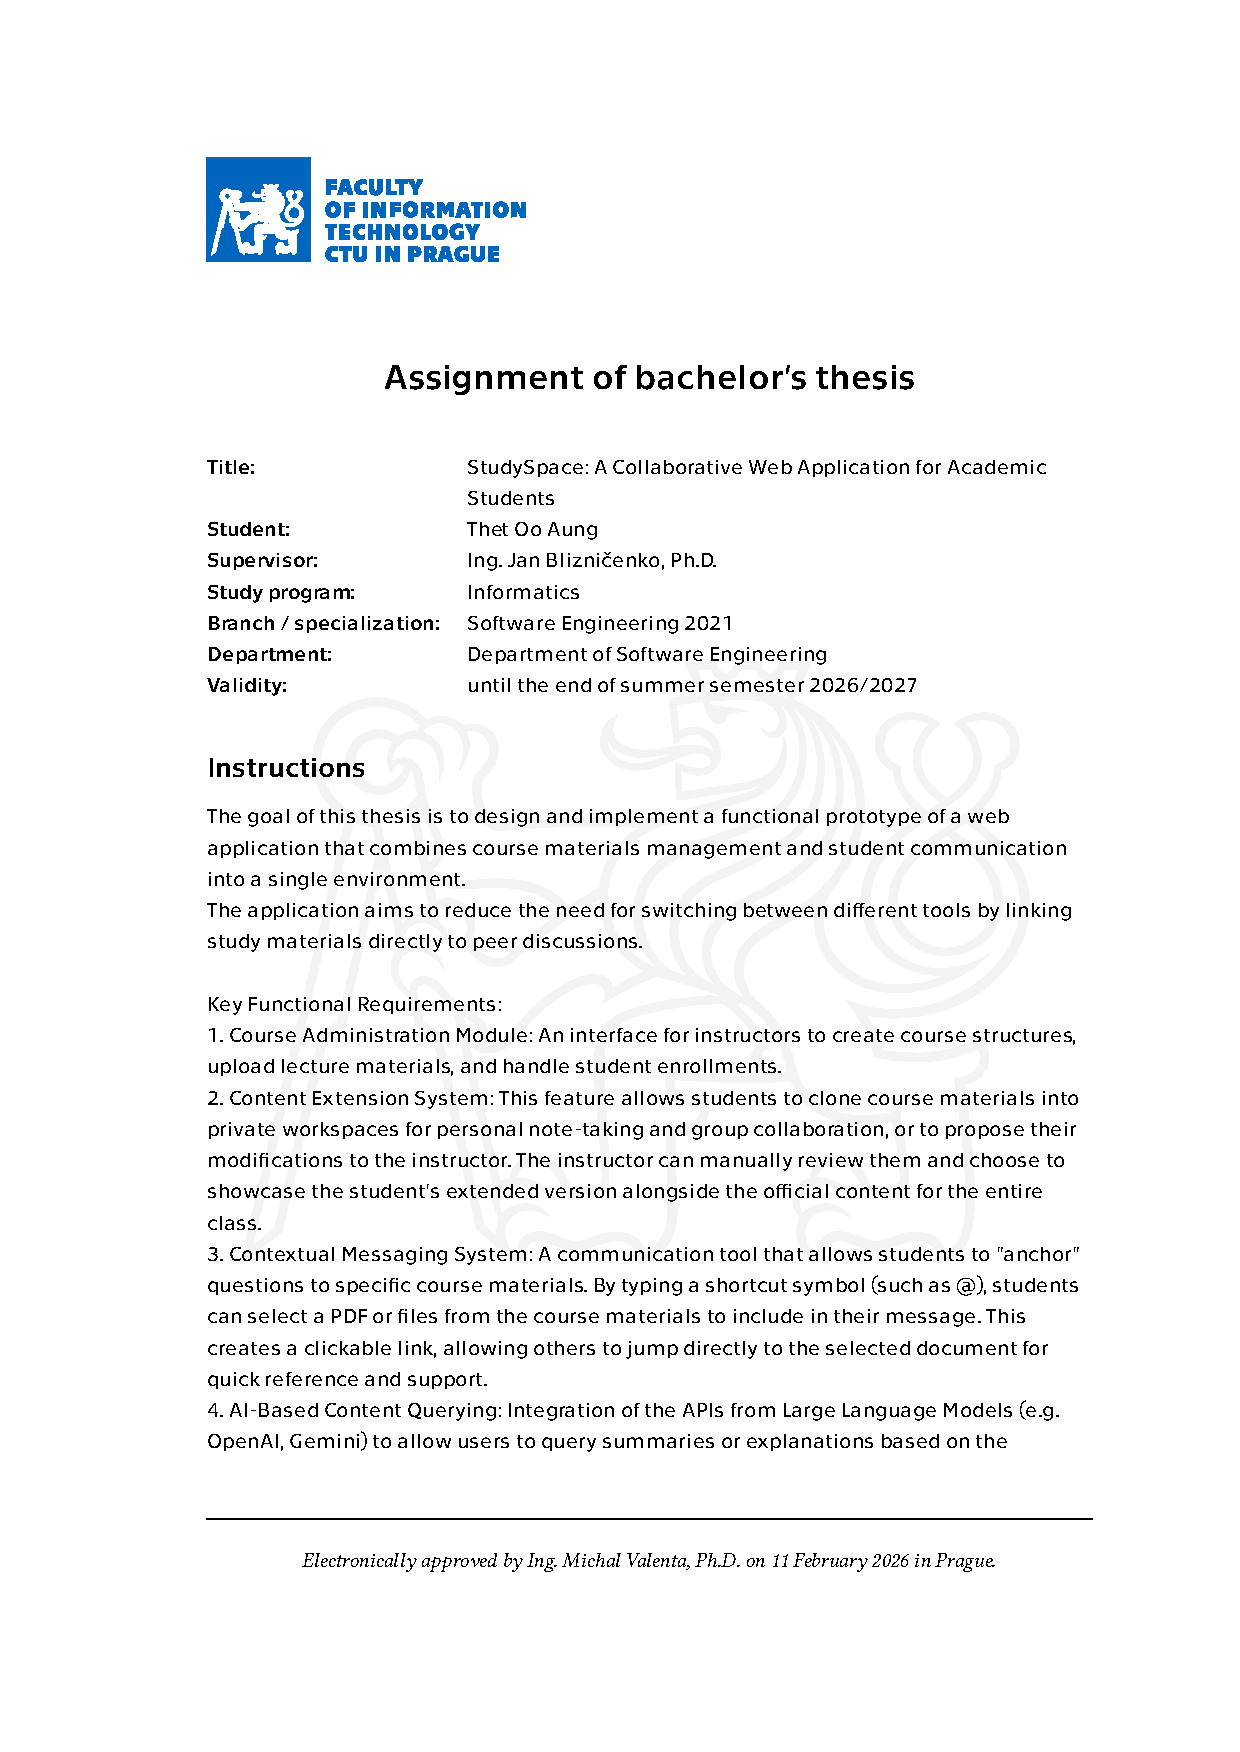
\includepdf[pages={1-}]{aungthet-assignment.pdf} % replace this file with your thesis assignment generated from ProjectsFIT

\imprintpage % do not remove this command
\stopTOCentries

%%%%%%%%%%%%%%%%%%%
% ACKNOWLEDGMENT
% FILL IN / MODIFY
% This is a place to thank people for helping you. It is common to thank your supervisor.
%%%%%%%%%%%%%%%%%%%
\begin{acknowledgmentpage}
	I would like to thank my supervisor, Ing. Jan Blizničenko, Ph.D., for his guidance throughout the preparation of this thesis. I would also like to thank my family for their continuous support and encouragement.
\end{acknowledgmentpage}
%%%%%%%%%%%%%%%%%%%
% ACKNOWLEDGMENT END
%%%%%%%%%%%%%%%%%%%


%%%%%%%%%%%%%%%%%%%
% DECLARATION
% FILL IN / MODIFY
%%%%%%%%%%%%%%%%%%%
% INSTRUCTIONS
% ENG: choose one of approved texts of the declaration. DO NOT CREATE YOUR OWN. Find the approved texts at https://courses.fit.cvut.cz/SFE/download/index.html#_documents (document Declaration for FT in English)
% CZE/SLO: Vyberte jedno z fakultou schvalenych prohlaseni. NEVKLADEJTE VLASTNI TEXT. Schvalena prohlaseni najdete zde: https://courses.fit.cvut.cz/SZZ/dokumenty/index.html#_dokumenty (prohlášení do ZP)
\begin{declarationpage}
	I hereby declare that this bachelor’s thesis entitled “StudySpace” was written by me independently and that I have used only the sources listed in the bibliography. I declare that I have not submitted this thesis or any part thereof for the purpose of obtaining any other degree or qualification.
	
	I acknowledge that my thesis is subject to the Act No. 121/2000 Coll., the Copyright Act of the Czech Republic, and that Czech Technical University in Prague has the right to conclude a license agreement on the use of this thesis
as specified by this Act.
\end{declarationpage}
%%%%%%%%%%%%%%%%%%%
% DECLARATION END
%%%%%%%%%%%%%%%%%%%

% Use one of the two following commands. The first prints abstracts+keywords on two pages, the second puts them on one page (if possible). \printonepageabstract can also accept optional argument that specifies a vertical space before both abstracts (the default is 18 mm).
\printtwopageabstract
%\printonepageabstract

\tableofcontents % do not remove this command
%%%%%%%%%%%%%%%%%%%%%%
% list of other contents: figures, tables, code listings, algorithms, etc.
% add/remove commands accordingly
%%%%%%%%%%%%%%%%%%%%%%
\listoffigures % list of figures
\begingroup
\let\clearpage\relax
\listoftables % list of tables. Remove if you do not have any.
\thectufitlistingscommand{} % list of code listings. Remove if you do not have any.
\thectufitlistofalgorithmscommand{} % list of algorithm pseudocodes defined using the algorithm package.
\endgroup
%%%%%%%%%%%%%%%%%%%%%%
% list of other contents END
%%%%%%%%%%%%%%%%%%%%%%

%%%%%%%%%%%%%%%%%%%
% ABBREVIATIONS
% FILL IN / MODIFY
% OR REMOVE ENTIRELY
% List the abbreviations in lexicography order.
%%%%%%%%%%%%%%%%%%%
\chapter{\thectufitabbreviationlabel}

\begin{tabular}{rl}
	API   & Application Programming Interface              \\
	CS    & Computer Science                               \\
	DB    & Database                                       \\
	DTO   & Data Transfer Object                           \\
	ER    & Entity-Relationship                            \\
	HTTP  & Hypertext Transfer Protocol                    \\
	JPA   & Java Persistence API                           \\
	JSON  & JavaScript Object Notation                     \\
	JWT   & JSON Web Token                                 \\
	LLM   & Large Language Model                           \\
	LMS   & Learning Management System                     \\
	MVC   & Model-View-Controller                          \\
	ORM   & Object-Relational Mapping                      \\
	RAG   & Retrieval-Augmented Generation                 \\
	RBAC  & Role-Based Access Control                      \\
	REST  & Representational State Transfer                \\
	SPA   & Single Page Application                        \\
	SQL   & Structured Query Language                      \\
	SSR   & Server-Side Rendering                          \\
	UI    & User Interface                                 \\
	URL   & Uniform Resource Locator                       \\
	UX    & User Experience                                \\
	UML   & Unified Modeling Language                      \\
\end{tabular}
%%%%%%%%%%%%%%%%%%%
% ABBREVIATIONS END
%%%%%%%%%%%%%%%%%%%
\resumeTOCentries
\mainmatter\mainmatterinit % do not remove these two commands
%%%%%%%%%%%%%%%%%%%
% THE THESIS
% MODIFY ANYTHING BELOW THIS LINE
%%%%%%%%%%%%%%%%%%%

%% This file serves as the main entry point for all of your chapters.
%% Instead of writing everything here, we organize the thesis by
%% inputting individual chapter files from the `text/` directory sequentially.

\chapter{Introduction}
\label{ch:introduction}

Imagine a student preparing for an exam at the Faculty of Information Technology at CTU in Prague.
She has a question about a specific diagram on slide 14 of the lecture notes uploaded to the faculty
course system. To ask her peers, she must switch to Discord, copy the name of the file from the
course page, paste it into a message, and hope that her classmates can locate the same slide quickly
enough to give a useful answer. The question floats away in the message history by the next morning,
disconnected from the material it was about and invisible to students who enrol in the course the
following semester. This scenario, repeated across every course and every cohort, illustrates the
fundamental problem that StudySpace is designed to address: the fragmentation of academic tools that
forces students and instructors to operate across multiple disconnected platforms.

% ----------------------------------------------------------------
\section{Motivation}
\label{sec:motivation}

Modern higher education relies on a combination of platforms that rarely communicate with one
another. At a typical faculty, course materials reside in a learning management system such as Moodle
or the faculty course portal, while student collaboration happens informally on Discord, WhatsApp, or
Microsoft Teams. Code assignments and grading are handled by yet another system, and AI tools such
as ChatGPT are used in isolation without any link to the actual curriculum content. The consequence
of this fragmentation is that information ends up scattered: a useful correction that a student
discovers during self-study has no path back into the course, a question about a specific document
carries no reference to the document itself, and knowledge generated by one cohort is invisible to
the next.

StudySpace addresses these gaps by combining four capabilities in a single environment. Instructors
need a structured way to organise and publish course materials and to manage which students can
access them (F1). Students, rather than passively consuming that content, need a mechanism to clone
a workspace, enrich it with their own notes, and contribute improvements back to the original course
page for the instructor to review and optionally publish (F2). When students want to ask a question
about a specific document, they need a messaging channel that can attach a direct reference to that
document, so other readers can follow the link and land on the relevant material immediately (F3).
Finally, students need an AI assistant that queries the actual course content rather than operating
on general knowledge alone, grounding answers in the material the instructor has provided (F4). All
of these capabilities require a role-based access model that distinguishes instructors from students
at the API level, preventing students from modifying course materials they do not own (F5).

% ----------------------------------------------------------------
\section{Structure}
\label{sec:structure}

Chapter~\ref{ch:analysis} defines the target audience and their pain points, establishes the
functional and non-functional requirements derived from the motivation above, examines existing
platforms and their limitations, and describes the planned system and logical architecture.
Chapter~\ref{ch:design} translates the analysis into concrete technical decisions, covering the
domain model, the technology choices and the rationale behind each, the database schema, and the
user interface design.
Chapter~\ref{ch:implementation} documents the implementation of the five core features, presents
the code listings that illustrate the most important design choices, and describes how the system
was tested.
Chapter~\ref{ch:conclusion} summarises the outcomes relative to the goals stated in this chapter,
reflects on the known limitations of the prototype, and proposes directions for future work.

\chapter{Analysis}
\label{ch:analysis}

This chapter establishes the foundation for all subsequent design and implementation decisions.
It begins by defining the problem and the target audience whose needs motivated this project, then
describes the intended architecture at a conceptual level before any technology is named. The formal
functional and non-functional requirements are stated next, followed by a use-case view grouped by
actor. The chapter closes by examining existing platforms and identifying the integration gap that
none of them currently fills.

% ----------------------------------------------------------------
\section{Problem Statement and Target Audience}
\label{sec:problem-statement}

The primary target audience of StudySpace consists of two groups whose workflows are closely
coupled: \emph{students} and \emph{instructors} at a higher-education faculty. Students are the
consumers and potential contributors of course content. Their typical lifecycle within a single
course involves browsing uploaded materials, asking questions about specific documents, annotating
or extending study notes independently, and occasionally contributing improvements that could
benefit their peers. Instructors are the publishers and curators of that content. Their lifecycle
involves creating a course structure, uploading materials into named sections, managing which
students are enrolled, and reviewing any student contributions before deciding whether to make them
visible to the whole class.

The Faculty of Information Technology at CTU in Prague serves as the representative context. A
student's daily workflow involves switching between multiple systems: the faculty course portal or
Moodle for lecture slides and reading assignments, Microsoft Teams or SharePoint for live sessions
and recordings, Progtest or GitLab for programming assignments and grading, and Discord, WhatsApp,
or email for informal peer discussion. This constant context-switching leads to scattered
information, loss of peer-generated knowledge, and extra effort spent locating the right tool for a
given task. Discussions about a specific lecture slide happen in a general chat channel with no link
to the actual material. Student notes and annotations remain in personal files and never contribute
back to the course. There is no structured way for a student to propose improvements to lecture
materials, and AI tools are used in isolation without any connection to the course content.

StudySpace aims to unify course management, student collaboration, contextual discussion, and AI
assistance into a single platform, so that the interactions between these activities are preserved
and visible to all participants.

% ----------------------------------------------------------------
\section{Architecture Overview}
\label{sec:architecture-overview}

\subsection{System Architecture}
\label{subsec:system-architecture}

At the highest level, StudySpace is a web application that separates the browser-based user
interface from the server-side application logic and the persistent data store. The user interface
runs entirely in the browser and communicates with the backend over two channels: a standard
request-response channel for operations such as loading course content, uploading materials, and
submitting contribution proposals, and a persistent real-time channel for events that must reach
all connected participants without a manual page refresh, such as chat messages and study-session
activity feeds.

The backend is a single application that handles all business logic, enforces access control,
processes file uploads, calls the external AI API, and broadcasts real-time events. The data store
holds all persistent state, including user accounts, course structures, Private Workspace records,
Merge Proposals, and conversation history.

All three tiers run as isolated containers managed by a single container orchestration file, so the
complete application can be started with one command and requires no manual environment
configuration. The final architecture diagram is presented in section~\ref{sec:system-architecture-final}
after the technology choices have been made.

% TODO: Insert high-level system architecture diagram here
% \begin{figure}[htbp]
%     \centering
%     \includegraphics[width=0.9\textwidth]{images/fig_2_1_system-architecture.png}
%     \caption{Conceptual three-tier system architecture of StudySpace}
%     \label{fig:conceptual-architecture}
% \end{figure}

\subsection{Logical Architecture}
\label{subsec:logical-architecture}

The server-side application follows the Model-View-Controller (MVC) layered pattern. The
\emph{controller layer} receives HTTP requests, delegates to the appropriate service, and serialises
the response. The \emph{service layer} contains all business logic, orchestrates data access, and
enforces domain rules such as ownership checks and status transitions. The \emph{repository layer}
provides data access through named query methods and custom queries for complex lookups. Entity
classes map the relational schema to Java objects. Data Transfer Objects (DTOs) define the API
contract and decouple the internal entity structure from the shape of the JSON responses, so the
two can evolve independently.

% TODO: Insert MVC layered architecture diagram here
% \begin{figure}[htbp]
%     \centering
%     \includegraphics[width=0.85\textwidth]{images/fig_2_2_logical-architecture.png}
%     \caption{Logical (MVC) architecture of the StudySpace backend}
%     \label{fig:logical-architecture}
% \end{figure}

% ----------------------------------------------------------------
\section{Functional Requirements}
\label{sec:requirements}

The following requirements are derived directly from the problem statement and the target audience
description in section~\ref{sec:problem-statement}. Each requirement is identified by an ID that
is referenced throughout the remainder of the thesis.

\bigskip
\noindent\textbf{FR-01 --- Course Administration.}
An Instructor must be able to create, update, and delete courses and organise their content into
named sections, while a Student must be able to browse and read any course they are enrolled in.

The Instructor creates a course with a title and description and controls whether it is published
and visible to students. Within a published course the Instructor defines \emph{sections}, each
with an ordered index that determines the display sequence. Course Materials (PDF documents,
slide sets, video files, or images) are uploaded into sections; the backend infers the file type
from the MIME type and extension and stores it alongside the file URL so the frontend can render
the appropriate viewer without an additional request. Enrollment is managed per student: the
Instructor can activate or drop individual students, and a student sees only the courses in which
their enrollment status is \texttt{ACTIVE}.

\bigskip
\noindent\textbf{FR-02 --- Content Extension System.}
A Student must be able to clone a course into a Private Workspace, add or modify materials
independently, and submit a Merge Proposal for the Instructor to review and optionally publish.

When a student clones a course, the backend performs a deep copy of the course structure into a
new \texttt{StudentWorkspace}: every section and every Course Material is mirrored as a
\texttt{WorkspaceSection} and a \texttt{WorkspaceMaterial}. Cloned materials carry the flag
\texttt{isReference = true}, meaning they point to the original file URL rather than a new copy,
which saves storage. The student may then upload additional materials into the Private Workspace.
When satisfied, the student submits a Merge Proposal, which the Instructor reviews in a dedicated
queue. On approval, the backend copies the student's file into the course storage and publishes it
as a new Course Material credited to the contributor.

\bigskip
\noindent\textbf{FR-03 --- Contextual Messaging System.}
Users must be able to post messages in the workspace chat and attach a direct reference to a
specific Course Material, so that other users can open the material from within the message.

The chat panel is embedded in the workspace view alongside the material list. Users compose
messages in a rich-text input and can type \texttt{@} followed by a material name to trigger an
autocomplete dropdown. Selecting a material embeds a non-editable tag chip in the message. When
the message is submitted, the chip is serialised into a portable token of the form
\texttt{@[id:title]}, which is stored as the message text. On render, the token is parsed back into
a clickable badge, which the user clicks to download or open the referenced Course Material. This
Contextual Anchor persists in the chat history and remains accessible to every enrolled student who
opens the workspace later.

\bigskip
\noindent\textbf{FR-04 --- AI-Based Content Querying.}
Users must be able to ask natural-language questions about the content of the currently open
workspace and receive answers grounded in that content.

The AI panel is a collapsible sidebar within the workspace view. When the user submits a question,
the frontend sends the question together with the URL of the selected Course Material to the
backend. The backend extracts the plain text from the document, constructs a structured prompt
that includes a system instruction, the document context truncated to 10\,000 characters, and the
user's question, then forwards the prompt to the Large Language Model (LLM) API. The response is
streamed back to the frontend and displayed with a typewriter animation. Conversation history is
preserved in the database through a hybrid memory model: a rolling buffer of recent messages and a
compressed long-term summary, ensuring that the AI can reference earlier turns in a session even
after the short-term buffer overflows.

\bigskip
\noindent\textbf{FR-05 --- Access Control.}
The system must recognise two roles, Student and Instructor, and enforce role-based restrictions
at the API level so that students cannot perform instructor-only operations.

Role assignment happens at registration and is stored as the \texttt{role} field of the
\texttt{User} entity. The authentication flow issues a signed JSON Web Token (JWT) upon successful
login; the token encodes the user's email and is valid for ten hours. Every subsequent request must
carry the token in the \texttt{Authorization: Bearer} header. The \texttt{JwtAuthenticationFilter}
intercepts each request, extracts and validates the token, and populates the Spring Security
context. Instructor-only endpoints are protected with \texttt{@PreAuthorize} annotations or
explicit ownership checks in the service layer so that a student account receives an HTTP 403
response if it attempts a restricted operation.

\subsection{Non-Functional Requirements}
\label{subsec:nonfunctional-requirements}

The following non-functional requirements define the quality constraints the system must satisfy
regardless of the specific feature being used.

\begin{table}[htbp]
    \centering
    \caption{Non-functional requirements}
    \label{tab:nonfunctional-requirements}
    \renewcommand{\arraystretch}{1.4}
    \begin{tabularx}{\textwidth}{|p{1.5cm}|X|}
        \hline
        \textbf{ID} & \textbf{Description} \\
        \hline
        NFR-01 & \textbf{Usability}: The interface should be straightforward enough for
                 students with no prior training to use without a manual. \\
        \hline
        NFR-02 & \textbf{Security}: All endpoints except login and registration must
                 require a valid JWT token. Role-based access must be enforced on the
                 server side. \\
        \hline
        NFR-03 & \textbf{Performance}: Course and workspace pages should load within
                 three seconds under normal conditions. \\
        \hline
        NFR-04 & \textbf{Maintainability}: The backend and frontend must be clearly
                 separated and independently deployable. The project structure should
                 follow established conventions for its respective framework. \\
        \hline
        NFR-05 & \textbf{Deployability}: The entire application must be runnable with
                 a single Docker Compose command without manual environment setup. \\
        \hline
    \end{tabularx}
\end{table}

% ----------------------------------------------------------------
\section{Use Cases}
\label{sec:use-cases}

The system has two types of actors: \emph{Student} and \emph{Instructor}. The use cases below
describe the main interactions each actor has with the system, grouped by role. Pre-conditions
are stated for the non-trivial cases that have dependencies on prior system state.

% TODO: Insert use case diagram here
% \begin{figure}[htbp]
%     \centering
%     \includegraphics[width=0.9\textwidth]{images/fig_2_3_use-case-diagram.png}
%     \caption{UML use case diagram for StudySpace}
%     \label{fig:use-case-diagram}
% \end{figure}

\subsection*{Instructor Use Cases}

\begin{itemize}
    \item \textbf{\texttt{Create course}}: The Instructor creates a course with a title and
          description and sets its published status.
    \item \textbf{\texttt{Upload Course Material}}: Pre-condition: the course and at least one
          section exist. The Instructor selects a file, assigns a title, and uploads it into a
          named section. The backend infers the file type and persists the file URL.
    \item \textbf{\texttt{Manage enrolments}}: The Instructor approves or drops individual
          student enrollments from the course management panel.
    \item \textbf{\texttt{Review Merge Proposal}}: Pre-condition: at least one student has
          submitted a Merge Proposal for this course. The Instructor inspects the proposed
          Course Material and either approves it (publishing it on the main course page with the
          contributor's name attached) or rejects it with an optional review note.
\end{itemize}

\subsection*{Student Use Cases}

\begin{itemize}
    \item \textbf{\texttt{Browse course materials}}: The student navigates to an enrolled course
          and opens individual sections to read the uploaded Course Materials.
    \item \textbf{\texttt{Clone course to Private Workspace}}: Pre-condition: the student is
          enrolled in a published course. The student triggers a clone action; the backend creates
          a Private Workspace containing mirror copies of all sections and Course Materials.
    \item \textbf{\texttt{Submit Merge Proposal}}: Pre-condition: the student owns a Private
          Workspace with at least one non-reference material or a modified reference material.
          The student selects materials and a target section, optionally adds a message, and
          submits the proposal for Instructor review.
    \item \textbf{\texttt{Post contextual message}}: The student types a message in the workspace
          chat, uses \texttt{@} to attach a Contextual Anchor to a specific Course Material, and
          submits. All enrolled users can see the message and follow the anchor.
    \item \textbf{\texttt{Query AI assistant}}: The student opens the AI panel, selects a Course
          Material for context, and types a question. The system sends the question and the
          extracted document text to the LLM API and displays the answer.
\end{itemize}

% ----------------------------------------------------------------
\section{Existing Solutions}
\label{sec:existing-solutions}

Several platforms address parts of the problem described in section~\ref{sec:problem-statement}.
This section compares the most relevant ones against the core features that StudySpace provides,
concluding with a synthesis of the integration gap that none of them fills end-to-end.

\begin{table}[htbp]
    \centering
    \small
    \caption{Comparison of existing platforms against StudySpace features}
    \label{tab:platform-comparison}
    \renewcommand{\arraystretch}{1.4}
    \begin{tabularx}{\textwidth}{>{\raggedright\arraybackslash}p{1.5cm} *{5}{>{\centering\arraybackslash\hspace{0pt}}X}}
        \toprule
        \textbf{Platform}
            & \textbf{Structured course materials}
            & \textbf{Student content contribution}
            & \textbf{Contextual discussion}
            & \textbf{AI content assistance}
            & \textbf{Role-based access control} \\
        \midrule
        \textbf{Zoom / Teams}
            & None & None & None & None & Partial \\
        \textbf{Discord}
            & None & None & None & None & Partial \\
        \textbf{Moodle}
            & Full & Limited & None & None & Full \\
        \textbf{Notion / Docs}
            & Full & Partial & None & Generic & None \\
        \textbf{StudySpace}
            & Full & Full & Full & Context & Full \\
        \bottomrule
    \end{tabularx}
\end{table}

The comparison in Table~\ref{tab:platform-comparison} shows that no existing platform covers all
areas simultaneously. The following subsections analyse each platform in detail.

% ----------------------------------------------------------------
\subsection{Zoom and Microsoft Teams}
\label{subsec:zoom-teams}

Zoom and Microsoft Teams are the dominant platforms for synchronous online education. Both support
high-quality video conferencing, screen sharing, breakout rooms, and session recording. Microsoft
Teams adds persistent channels, a file-sharing area backed by SharePoint, and deep integration
with the Microsoft 365 productivity suite.

Despite these strengths, neither platform is designed for asynchronous, material-centric
collaboration. Files shared during a meeting are stored in a flat SharePoint folder rather than
being organised into a course structure that reflects the academic curriculum. Discussion threads
are tied to meeting events, making conversations about a lecture slide inaccessible to students
who join the course later. There is no mechanism for students to annotate shared files and propose
changes back to the Instructor; the Instructor remains the sole publisher of content. The
asynchronous knowledge-management and student contribution use cases are left entirely unaddressed.

% ----------------------------------------------------------------
\subsection{Discord}
\label{subsec:discord}

Discord was originally designed for gaming communities but has been widely adopted by student
groups as an informal alternative to institutional platforms. Its server and channel model allows
students to self-organise into topic-specific channels, and its low barrier to entry means that
most students already have an account.

However, Discord's design is fundamentally chat-centric and lacks any concept of structured
educational content. Files are posted as raw message attachments in a general channel with no link
to a course section or curriculum structure. There is no role hierarchy that distinguishes
Instructors from students at the permission level beyond basic moderation roles; an Instructor
cannot publish a set of Course Materials in a read-only area that students can then clone and
annotate. Content disappears into scroll history, there is no access control aligned with course
enrolment, and there is no mechanism for structured content contribution or AI-assisted querying
of Course Materials.

% ----------------------------------------------------------------
\subsection{Moodle}
\label{subsec:moodle}

Moodle is a mature, open-source Learning Management System (LMS) used by thousands of
universities worldwide, including CTU. It provides the most comprehensive course management
feature set of any platform considered: Instructors can define courses with hierarchical sections,
upload files and links, set up graded assignments and quizzes, track student progress, and manage
enrolment through a role-based permission model.

Despite this breadth, Moodle has well-documented limitations with respect to student agency and
contextual collaboration. Its discussion model is based on forums that are standalone modules
attached to a course but not anchored to specific Course Materials; a student cannot attach a
comment directly to a particular document without navigating to a separate forum module. Student
contribution in Moodle is limited to wiki modules and assignment submissions, which are graded
artefacts that do not become part of the course content visible to other students. Moodle also
has no built-in AI assistant that operates on the actual course content in real time.

% ----------------------------------------------------------------
\subsection{Notion and Google Docs}
\label{subsec:notion-docs}

Notion and Google Docs represent a different category: general-purpose collaborative writing
tools. Both support real-time co-editing, rich text formatting, embedded media, and comment
threads. Notion extends this with a hierarchical page structure and customisable database views,
making it possible to approximate a course workspace.

The critical gaps are the absence of role-based access control aligned with academic roles and
the lack of a structured contribution workflow. In a shared Notion workspace, any collaborator
can edit any page, creating conflicts and the risk of accidental data loss in a course setting
with many students. Google Docs has stricter permission levels but no multi-tier workflow where a
student creates a private draft, develops it independently, and then submits it for review and
publication. Neither platform is AI-aware in a course-content sense: Notion AI and Google's
Gemini integration can generate or summarise text, but they operate on the open document in
isolation, without knowledge of which course the document belongs to or what other materials are
in the same section.

% ----------------------------------------------------------------
\subsection{Summary of Gaps}
\label{subsec:gap-summary}

The analysis above reveals a consistent pattern across all evaluated platforms. None of them
provides a mechanism for anchoring a discussion message to a named Course Material within a
structured course hierarchy, meaning that contextual references must be described manually in
text and the connection to the source material is easily lost. No platform supports a
clone-then-propose contribution model in which a student creates a private enriched copy of a
course section and submits it back for Instructor review and publication; the Instructor remains
the sole publisher of course content in every platform examined. Where AI assistance is
available, as in Notion AI or Google's Gemini integration, it operates on the open document in
isolation and cannot be grounded in the broader course context. The result is that satisfying all
four requirements simultaneously forces students to use at least two to three separate platforms,
reproducing the context-switching overhead described in section~\ref{sec:problem-statement}.

StudySpace addresses this integration gap by combining structured course management, a
clone-based student contribution workflow with Instructor review, chat messages with Contextual
Anchors tied to specific Course Materials, and an AI assistant grounded in the actual course
content, all within a single application with role-based access control.

\chapter{Design}
\label{ch:design}

This chapter translates the requirements and architectural overview established in
Chapter~\ref{ch:analysis} into concrete technical decisions. The domain model defines the
entities and their relationships. The technology analysis justifies each major component of the
stack by comparing alternatives against the project requirements. The database schema and
entity-relationship diagram document the persistent data model. The finalised system architecture
and API design are presented, and the chapter closes with the user interface design.

% ----------------------------------------------------------------
\section{Domain Model}
\label{sec:domain-model}

The domain model consists of the entities that carry the application's persistent state. Each
entity is described below, and the complete UML class diagram is presented in
Figure~\ref{fig:uml-class-diagram} at the end of this section.

\textbf{User} is the central actor entity. It stores the account credentials (username, email,
and bcrypt-hashed password), the display name, a profile picture URL, and a role field that
takes one of two values: \texttt{STUDENT} or \texttt{INSTRUCTOR}. The entity also tracks a
cumulative study-time counter and a current-streak counter that are updated by the gamification
subsystem. A user can create many \texttt{Course} records (as an Instructor), own many
\texttt{StudentWorkspace} records (as a Student), and participate in many \texttt{StudySession}
records through the \texttt{SessionParticipant} junction entity.

\textbf{Course} represents a published course created by one Instructor. It carries a title, a
text description, a boolean \texttt{isPublished} flag that controls student visibility, and a
many-to-one relationship to its owning \texttt{User} (the Instructor). Deleting a
\texttt{Course} cascades to all its \texttt{CourseSection} and \texttt{CourseEnrollment} records
via \texttt{CascadeType.ALL} with orphan removal, ensuring no orphaned sections or enrollments
remain after a course is removed.

\textbf{CourseSection} organises Course Materials within a course into named, ordered groups. It
carries a title, an optional text description, and an \texttt{orderIndex} integer that determines
the display sequence. Each section belongs to exactly one \texttt{Course}, and each section owns
an ordered list of \texttt{CourseMaterial} records. Deleting a section cascades to all its
materials.

\textbf{CourseMaterial} represents a single file uploaded into a course section. It stores a
display title, the file storage URL, the inferred file type as a \texttt{MaterialType} enum
(\texttt{PDF}, \texttt{SLIDES}, \texttt{VIDEO}, \texttt{IMAGE}, \texttt{OTHER}), the original
filename, an optional \texttt{contributorName} field (populated when the material originated
from an approved Merge Proposal), and a timestamp. Each \texttt{CourseMaterial} belongs to
exactly one \texttt{CourseSection}.

\textbf{CourseEnrollment} is the join entity that records a student's membership in a course.
It carries an \texttt{EnrollmentStatus} field (\texttt{ACTIVE} or \texttt{DROPPED}) and the
timestamp of the initial enrollment. A unique constraint on the pair \texttt{(course\_id,
student\_id)} prevents duplicate enrollment rows. Setting the status to \texttt{DROPPED} rather
than deleting the row preserves the enrollment history and allows re-activation.

\textbf{StudentWorkspace} is the root entity of a student's Private Workspace. It holds a name,
a description, a reference to the owning \texttt{User}, and a list of \texttt{WorkspaceSpace}
records. The workspace is the container that the student manages independently; it does not belong
to any course and cannot be seen or modified by the Instructor.

\textbf{WorkspaceSpace} represents a single cloned or manually created space within a Private
Workspace. It carries a title, a description, an optional foreign key to the \texttt{Course} it
was forked from (\texttt{forkedFromCourse}), and a boolean \texttt{isPublished} flag used when a
space is surfaced in a public gallery. Each space owns an ordered list of
\texttt{WorkspaceSection} records.

\textbf{WorkspaceMaterial} mirrors \texttt{CourseMaterial} within the student's space. Two flags
encode the copy-on-write behaviour: \texttt{isReference = true} means the material points to
the original course file URL and no physical copy was made; \texttt{isHidden = true} implements
a soft-delete that hides the row from the student's view without physically removing it, which is
necessary because a contribution proposal may hold a foreign-key reference to the material row
and deleting it would violate referential integrity.

\textbf{ContributionProposal} links a student's \texttt{WorkspaceMaterial} to a target
\texttt{Course} and optionally a target \texttt{CourseSection}. Its \texttt{ProposalStatus} enum
field (\texttt{PENDING}, \texttt{APPROVED}, \texttt{REJECTED}) drives the Instructor review
workflow. When no existing section is targeted, the \texttt{proposedSectionTitle} field holds the
name of a new section to be created on approval. The \texttt{reviewedAt} timestamp is set when
the Instructor takes action, and the \texttt{contributorDisplayName} is copied from the student's
profile at submission time so it remains stable even if the student later changes their name.

\textbf{Conversation} persists the AI chat memory for a single user session. Rather than storing
every message individually in a separate table, the entity uses a hybrid memory model: a
\texttt{summary} text column holds a compressed rolling summary of older turns, updated by a
separate LLM call when the recent buffer overflows, and a \texttt{recentMessages} column stores
a JSON-serialised list of the most recent turns as plain text (compatible with PostgreSQL
\texttt{TEXT} and H2 for testing). The entity's primary key is a client-generated UUID string,
so no database sequence is required.

% TODO: Insert UML class diagram as Figure 3.1
% \begin{figure}[htbp]
%     \centering
%     \includegraphics[width=\textwidth]{images/fig_3_1_uml-class-diagram.png}
%     \caption{UML class diagram of the StudySpace domain model}
%     \label{fig:uml-class-diagram}
% \end{figure}

% ----------------------------------------------------------------
\section{Technology Analysis}
\label{sec:technologies}

This section justifies each major technology choice by comparing the available alternatives against
the requirements established in Chapter~\ref{ch:analysis}. The goal was to select a stack that is
well suited for the required features, has strong community support and ecosystem maturity, and is
practical to use within the scope of a bachelor thesis prototype.

% ----------------------------------------------------------------
\subsection{Frontend Framework}
\label{subsec:frontend-tech}

FR-01 through FR-04 require a responsive, component-rich user interface that manages complex
shared state across a course-material viewer, a chat panel, and an AI assistant panel rendered
simultaneously on the same screen.

\textbf{React~19}~\cite{React} is a declarative UI library maintained by Meta. Its component model
encourages decomposing the interface into small, reusable pieces, each responsible for a single
part of the view. The unidirectional data flow makes state changes predictable and easier to trace
during debugging. React's large ecosystem provides ready-made solutions for drag-and-drop panels,
rich-text editing, and real-time subscriptions, all of which are needed for StudySpace.

\textbf{Vue.js} is a progressive framework with a smaller bundle size and a gentler learning
curve. For StudySpace, however, the Vue ecosystem is shallower for complex, enterprise-grade
components, and the TypeScript integration, while improving, is less seamless than in React.

\textbf{Angular} is a full-featured framework backed by Google that includes dependency injection,
a router, and a form library out of the box. The overhead of Angular's concepts, decorators, and
module system exceeds what is justified for a single-team prototype of this scope.

React was selected because its component model aligns directly with the StudySpace screen layout
(course panel, chat sidebar, AI panel as discrete components), its TypeScript support is
first-class, and its ecosystem provides the resizable panel, rich-text input, and WebSocket hook
primitives needed by FR-02 and FR-03 without significant additional integration effort.

React is used through the \textbf{Next.js~15}~\cite{Nextjs} framework, which provides file-based
routing via the App Router, server-side rendering where applicable, and built-in image
optimisation. Compared to a plain Vite or Create React App setup, Next.js removes boilerplate
routing configuration and makes the project structure self-documenting through the directory
layout. Styling is handled by \textbf{Tailwind CSS}~\cite{TailwindCSS} combined with
\textbf{Shadcn/ui}~\cite{ShadcnUI} and \textbf{Radix UI}, which provide accessible, unstyled
component primitives that Tailwind classes are applied to. State management across the application
uses \textbf{Redux Toolkit}~\cite{ReduxToolkit}, which offers predictable reducers and typed
async thunks for all API interactions.

% ----------------------------------------------------------------
\subsection{Backend Framework}
\label{subsec:backend-tech}

FR-05 requires robust authentication and role-based authorisation. FR-02 and FR-04 involve
complex transactional operations over relational data. These requirements favour a statically
typed language with mature transaction management and security libraries.

\textbf{Java~21 with Spring Boot~3}~\cite{Java21,SpringBoot} provides a statically typed,
object-oriented foundation with a mature ecosystem. Spring Boot's convention-over-configuration
approach applies sensible defaults automatically, embeds a Tomcat web server, and offers
first-class integration with Spring Security, Spring Data JPA, Spring WebSocket, and Springdoc
OpenAPI --- all of which are essential for StudySpace. Virtual Threads, introduced in Java~21,
improve the throughput of concurrent request handling without the complexity of reactive
programming.

\textbf{Node.js with NestJS or Express} excels in I/O-bound tasks due to its event-driven
architecture. However, its single-threaded event loop can be a bottleneck for the multi-step
transactional operations required by the Content Extension System (FR-02), and the ORM ecosystem
does not reach the integration depth and stability of Spring Data JPA.

\textbf{Python with Django or FastAPI} is excellent for rapid prototyping and AI integration.
Python's dynamic typing, however, makes maintaining large-scale backend codebases more challenging
without strict tooling, and its Global Interpreter Lock can become a bottleneck for highly
concurrent CPU-bound tasks.

Java~21 with Spring Boot~3 was selected because the controller-service-repository layered model
maps directly onto the StudySpace domain structure, Spring Security provides JWT-based
authentication and method-level authorisation out of the box (directly addressing FR-05), and the
mature transaction management ensures referential integrity across the complex clone and proposal
approval operations required by FR-02.

% ----------------------------------------------------------------
\subsection{Database and Vector Store}
\label{subsec:database-tech}

The application's data model is inherently relational: users own workspaces, workspaces belong
to courses, clone records track inheritance, and proposals reference both student materials and
instructor courses. FR-02 requires ACID transaction guarantees across multi-entity writes.

\textbf{PostgreSQL~17}~\cite{PostgreSQL} is a mature, open-source relational database management
system (RDBMS) that follows the SQL standard and supports complex queries, transactions, and
foreign key constraints. It integrates seamlessly with the Java backend through the JDBC driver,
and higher-level access is provided by Spring Data JPA with Hibernate as the ORM provider.

\textbf{MongoDB} (NoSQL document store) and \textbf{Cassandra} (wide-column store) are optimised
for unstructured or semi-structured data and horizontal scalability. However, they lack strict
schema enforcement and standard join operations. Using a document store would require significant
denormalisation, duplicating data to avoid application-level joins, which introduces the risk of
inconsistency when a Course Material is approved and must be reflected in both the workspace and
the course tables atomically.

PostgreSQL was selected because the StudySpace data model is fundamentally relational, ACID
transactions are required for the clone and approval workflows (FR-02), and foreign-key
constraints enforce referential integrity between proposals and their source materials. The AI
assistant (FR-04) does not require a dedicated vector store at this prototype stage because the
document text is extracted at query time and injected directly into the prompt; full vector
embeddings are identified as a future extension in section~\ref{sec:future-work}.

% ----------------------------------------------------------------
\subsection{LLM API Integration}
\label{subsec:ai-tech}

FR-04 requires an LLM API capable of answering questions grounded in a provided document context
within a single prompt, without fine-tuning.

\textbf{Google Gemini API (gemini-2.5-flash)} provides a large context window, competitive
quality on open-domain question answering, and an official Java SDK that integrates directly with
the Spring Boot application. The free tier is sufficient for prototype-level usage.

\textbf{OpenAI GPT-4o} exposes a compatible REST interface and achieves comparable quality on
question answering tasks. However, the Java SDK is less mature than the official Google GenAI
SDK, and the cost per token is higher for the same context window size at the time of writing.

The Google Gemini API was selected because the official Google GenAI Java SDK~\cite{GoogleGenAI}
integrates directly with Spring Boot without additional HTTP client configuration, the
\texttt{gemini-2.5-flash} model's context window comfortably accommodates the 10\,000-character
document extract required by FR-04, and the free tier capacity is sufficient for the prototype.

% ----------------------------------------------------------------
\subsection{Authentication and Authorisation}
\label{subsec:auth-tech}

FR-05 requires stateless authentication suitable for a REST API consumed by a single-page
application, with role-based restrictions enforced on the server side.

\textbf{JSON Web Tokens (JWT) with Spring Security}~\cite{SpringSecurity} enables stateless
authentication: after login, the server issues a signed token that the client stores and sends
with every subsequent request. The server validates the token signature without consulting a
session store, which simplifies horizontal scaling.

\textbf{Server-side sessions} with Spring Session require a shared session store (such as Redis)
across instances and add network latency to every request. For a stateless REST API served to a
browser-based SPA, this overhead is unnecessary.

\textbf{OAuth~2.0 only} (without local credentials) would prevent users without a Google or
GitHub account from registering, which is inappropriate for a faculty application where students
may not use third-party providers for academic accounts.

JWT with Spring Security was selected because it achieves stateless session management (directly
satisfying NFR-02), requires no external session store, and Spring Security's filter chain
integrates the JWT validation and role check into a single, reusable \texttt{OncePerRequestFilter}
implementation. Google OAuth~2.0 login is supported as an optional alternative authentication
path alongside the primary local credential flow.

% ----------------------------------------------------------------
\subsection{Real-Time Communication}
\label{subsec:websocket-tech}

The study-session feature requires real-time event delivery to all connected participants without
polling, as required by the real-time study-session feature.


\textbf{WebSocket with STOMP over SockJS}~\cite{SockJS} layers a publish-subscribe model on top
of the raw WebSocket connection. Spring Boot registers a broker endpoint and routes messages to
per-session topics, allowing the server to push participant-list updates and activity events to
all subscribers without the clients polling.

\textbf{Server-Sent Events (SSE)} provide a unidirectional push channel from server to client.
They lack the bidirectional subscription model needed for clients to send activity events (such as
a hand-raise) back to the server over the same connection.

\textbf{Long Polling} achieves real-time delivery but requires each client to maintain a pending
request and re-establish it after every response, producing significant per-client overhead on
the server.

WebSocket with STOMP over SockJS was selected because the bidirectional subscription model covers
both server-to-client pushes (participant list updates, activity events) and client-to-server
messages (hand raises) over a single connection, and Spring Boot's built-in STOMP message broker
requires no additional infrastructure.

% ----------------------------------------------------------------
\subsection{File Storage}
\label{subsec:storage-tech}

FR-01 and FR-02 require file upload and retrieval for Course Materials and Private Workspace
materials. The storage backend must be swappable between a local development mode and a
production cloud target.

\textbf{Local file storage} (writing files to a directory under the working directory) is zero-cost
and requires no external service in development. It is unsuitable for production because files are
lost when the container is recreated and cannot be shared across multiple server instances.

\textbf{Google Cloud Storage (GCS)} is a managed object store with high durability, direct URL
serving, and a Java client library. It requires a GCP project and credentials, which adds setup
overhead during development.

A \texttt{FileStorageService} interface with two concrete implementations was designed:
\texttt{LocalFileStorageService} for development and \texttt{GcsFileStorageService} for production.
The active implementation is selected by a Spring profile, keeping the storage backend transparent
to the rest of the application and satisfying NFR-04. The interface defines three methods:
\texttt{store}, \texttt{copy}, and \texttt{delete}, which are the only storage operations needed
by FR-01 and FR-02.

% ----------------------------------------------------------------
\section{Database Schema}
\label{sec:database-schema}

The relational schema follows directly from the domain model described in
section~\ref{sec:domain-model}. Each entity maps to a dedicated table, and all foreign-key
relationships are enforced at the database level.

The primary tables are \texttt{users}, \texttt{courses}, \texttt{course\_sections},
\texttt{course\_materials}, \texttt{course\_enrollments}, \texttt{student\_workspaces},
\texttt{workspace\_spaces}, \texttt{workspace\_sections}, \texttt{workspace\_materials},
\texttt{contribution\_proposals}, and \texttt{conversations}. The
\texttt{course\_enrollments} table carries a unique constraint on
\texttt{(course\_id, student\_id)} to prevent duplicate enrollment rows. The
\texttt{workspace\_materials} table carries the two boolean flags \texttt{isReference}
and \texttt{isHidden} that implement the copy-on-write and soft-delete semantics described
in section~\ref{sec:domain-model}.

The AI conversation memory is stored in the \texttt{conversations} table as two \texttt{TEXT}
columns: \texttt{summary} for the compressed long-term memory and \texttt{recent\_messages} for
the JSON-serialised short-term buffer. This design avoids a separate message table and keeps the
memory retrieval to a single row lookup by the client-generated UUID primary key. The current
prototype does not use vector embeddings; document text is extracted at query time and injected
into the prompt. A dedicated embedding column using \texttt{pgvector} is identified as a future
extension that would replace on-the-fly extraction with indexed similarity search.

% TODO: Insert ERD as Figure 3.2
% \begin{figure}[htbp]
%     \centering
%     \includegraphics[width=\textwidth]{images/fig_3_2_er-diagram.png}
%     \caption{Entity-relationship diagram of the StudySpace database schema}
%     \label{fig:er-diagram}
% \end{figure}

% ----------------------------------------------------------------
\section{System Architecture (Final)}
\label{sec:system-architecture-final}

StudySpace follows a three-tier architecture. The \emph{presentation layer} is a Next.js and
React application running in the browser; it communicates with the backend via the REST API for
most operations and via a persistent WebSocket (STOMP/SockJS) connection during active study
sessions. The \emph{business logic layer} is a Spring Boot application that handles authentication,
data access, real-time session broadcasting, and LLM API calls. The \emph{data layer} is a
PostgreSQL database that stores all persistent data.

All three tiers are defined in \texttt{docker-compose.yml} and run in the same Docker network,
so they can reach each other by service name without exposing internal ports to the host.

The backend is organised into the following packages, each with a single responsibility and
dependencies flowing only from controller to service to repository:

\begin{table}[htbp]
    \centering
    \caption{Backend package structure}
    \label{tab:backend-packages}
    \renewcommand{\arraystretch}{1.4}
    \begin{tabularx}{\textwidth}{|p{3cm}|X|}
        \hline
        \textbf{Package} & \textbf{Responsibility} \\
        \hline
        \texttt{controller} & Defines REST endpoints, maps HTTP requests to service calls,
                              and validates incoming request bodies. \\
        \hline
        \texttt{service} & Contains all business logic. Services are called by controllers
                          and may call one or more repositories. Transactions are managed
                          at this layer. \\
        \hline
        \texttt{repository} & Spring Data JPA repositories, providing CRUD operations and
                              custom JPQL queries for complex data access. \\
        \hline
        \texttt{entity} & JPA entity classes mapped to database tables. \\
        \hline
        \texttt{dto} & Data Transfer Objects used as the API contract, decoupling the
                      API response shape from the internal entity structure. \\
        \hline
        \texttt{security} & JWT filter, \texttt{UserDetailsService} implementation, and
                           Spring Security configuration. \\
        \hline
        \texttt{config} & Application-level configuration beans: CORS policy, Swagger
                         setup, and WebSocket registration. \\
        \hline
    \end{tabularx}
\end{table}

% TODO: Insert final architecture diagram as Figure 3.3
% \begin{figure}[htbp]
%     \centering
%     \includegraphics[width=0.9\textwidth]{images/fig_3_3_system-architecture-final.png}
%     \caption{Final system architecture of StudySpace}
%     \label{fig:system-architecture-final}
% \end{figure}

% ----------------------------------------------------------------
\section{API Design}
\label{sec:api-design}

The backend exposes a RESTful API following standard HTTP conventions. Resources are identified
by URL paths, and operations are expressed through HTTP methods (\texttt{GET}, \texttt{POST},
\texttt{PUT}, \texttt{DELETE}). All protected endpoints require a valid JWT token in the
\texttt{Authorization: Bearer <token>} header.

Authentication follows a four-step flow. The client sends credentials to
\texttt{POST /api/auth/login}. The server validates the credentials and returns a signed JWT
token. The client stores the token in memory and includes it in the \texttt{Authorization}
header of all subsequent requests. The server's \texttt{JwtAuthenticationFilter} validates the
token on each request before passing control to the controller.

The full API is documented through the Swagger UI available at \texttt{/swagger-ui/index.html}
when the backend is running, auto-generated by Springdoc OpenAPI from controller annotations.

% ----------------------------------------------------------------
\section{UI and Wireframe Design}
\label{sec:ui-design}

The interface is role-aware: students and Instructors see different navigation options and action
buttons depending on their role. The application uses a sidebar navigation layout with the main
content area to the right.

\subsection{Navigation and Layout}
\label{subsec:navigation}

The sidebar items differ by role. Students see links to their enrolled courses, their Private
Workspaces, and their study sessions. Instructors additionally see course management, enrollment
management, and Merge Proposal review links. The role check is performed client-side from the
JWT payload, but all data-sensitive actions are re-validated server-side.

\subsection{Course and Workspace Views}
\label{subsec:course-workspace-views}

The course list page shows all courses the user is enrolled in or manages. Selecting a workspace
opens the workspace viewer, which renders the Course Material alongside a contextual chat panel.
Students can use the chat panel to discuss the course content and attach a Contextual Anchor to
a specific Course Material using the \texttt{@}-mention system.

% TODO: Insert workspace view wireframe as Figure 3.4
% \begin{figure}[htbp]
%     \centering
%     \includegraphics[width=0.9\textwidth]{images/fig_3_4_workspace-view.png}
%     \caption{Workspace viewer wireframe: Course Material list with contextual chat panel}
%     \label{fig:workspace-view}
% \end{figure}

The workspace viewer places the material list on the left and the contextual chat panel on the
right. This layout satisfies the FR-03 use case \texttt{Post contextual message} by keeping the
source material and the discussion visible simultaneously. The panel is resizable so students can
balance reading space against chat space according to their preference.

\subsection{Private Workspace and Merge Proposal Views}
\label{subsec:clone-workspace}

When a student clones a course, they receive a Private Workspace that they can edit freely. The
cloned workspace view mirrors the course structure and adds upload controls for new materials.
The Merge Proposal submission dialog allows the student to select materials and choose a target
section, optionally typing a proposed new section name if none of the existing sections is
appropriate.

% TODO: Insert merge proposal wireframe as Figure 3.5
% \begin{figure}[htbp]
%     \centering
%     \includegraphics[width=0.9\textwidth]{images/fig_3_5_merge-proposal.png}
%     \caption{Merge Proposal submission dialog wireframe}
%     \label{fig:merge-proposal}
% \end{figure}

The Merge Proposal dialog reflects the FR-02 use case \texttt{Submit Merge Proposal}: the student
selects one or more materials, picks a target section or proposes a new one, and submits.
The design keeps the form minimal to reduce friction and mirrors the Git-inspired workflow that
technically experienced students will recognise.

\subsection{AI Assistant Panel}
\label{subsec:ai-panel}

The AI assistant is accessible through a collapsible side panel within the workspace viewer. The
student types a question in natural language, and the system sends the question together with
the content of the currently open Course Material to the LLM API. The response is displayed in
a conversational format with a typewriter animation. The panel is designed not to obscure the
Course Material so the student can consult both simultaneously.

% TODO: Insert AI panel wireframe as Figure 3.6
% \begin{figure}[htbp]
%     \centering
%     \includegraphics[width=0.85\textwidth]{images/fig_3_6_ai-panel.png}
%     \caption{AI assistant panel wireframe: question input and response display}
%     \label{fig:ai-panel}
% \end{figure}

The collapsible design satisfies FR-04 by making the AI assistant available at any point during
material review without forcing the student to navigate to a separate page, preserving the reading
context while the answer is displayed.

\chapter{Implementation}
\label{ch:implementation}

This chapter documents how the five core features defined in Chapter~\ref{ch:analysis} were
translated into working code. Each feature section follows the same structure: the purpose and
technical challenge are contextualised first, the application screenshot shows the feature in
action, the underlying logic is explained in prose, and a targeted code listing illustrates the
most important implementation decision. Section~\ref{sec:impl-testing} covers automated and
usability testing, and section~\ref{sec:impl-project-org} describes the project organisation.

% ----------------------------------------------------------------
\section{Course Administration Module (FR-01)}
\label{sec:impl-course}

The course administration feature addresses FR-01: Instructors must be able to create and manage
courses, upload Course Materials into named sections, and control student enrollment. The
technical challenge in this feature is keeping the file storage backend transparent to the
business logic so that the development environment (local disk) and the production environment
(Google Cloud Storage) can be swapped by changing a Spring profile, without any changes to the
service layer.

% TODO: Insert screenshot Figure 4.1
% \begin{figure}[htbp]
%     \centering
%     \includegraphics[width=0.9\textwidth]{images/fig_4_1_course-admin.png}
%     \caption{Instructor course management page: section list with upload controls}
%     \label{fig:course-admin}
% \end{figure}

The course management page presents the Instructor with a list of sections and a file upload
button per section. Selecting a file triggers a \texttt{multipart/form-data} request to the
backend; the Instructor does not see storage paths or file types, which are resolved automatically
by the backend.

The \texttt{CourseService} delegates all file operations to the \texttt{FileStorageService}
interface. When \texttt{uploadMaterial} is called, the service stores the file, infers the
\texttt{MaterialType} from the file extension, and persists the resulting URL in the
\texttt{CourseMaterial} entity. The ownership check in \texttt{assertInstructor} ensures that
only the course owner can modify sections or materials; any other authenticated user receives an
HTTP~403 response. The listing below shows the upload method, which encapsulates this flow in
under twenty lines.

\begin{lstlisting}[language=Java, caption={Code listing 4.1 --- Course material upload with storage abstraction (CourseService.java)}, label=lst:course-upload]
public CourseMaterialDTO uploadMaterial(
        Long sectionId, Long requestingUserId,
        MultipartFile file, String title) {
    CourseSection section = findSection(sectionId);
    // Only the course instructor may upload
    assertInstructor(section.getCourse(), requestingUserId);

    // FileStorageService is injected; impl selected by Spring profile
    String fileUrl = fileStorageService.store(file, "courses");
    MaterialType fileType = detectFileType(
            file.getOriginalFilename(), file.getContentType());

    CourseMaterial material = CourseMaterial.builder()
            .title(title).fileUrl(fileUrl)
            .fileType(fileType)
            .originalFileName(file.getOriginalFilename())
            .section(section).build();
    return toMaterialDTO(materialRepository.save(material));
}
\end{lstlisting}

The \texttt{FileStorageService} interface defines three methods (\texttt{store}, \texttt{copy},
\texttt{delete}), and the active implementation is injected by Spring. This design satisfies
NFR-04 (maintainability) by keeping the service layer unaware of the storage backend, and means
that switching to a cloud provider for production requires only an environment variable change,
not a code change.

% ----------------------------------------------------------------
\section{Content Extension System (FR-02)}
\label{sec:impl-fork}

The Content Extension System addresses FR-02: students must be able to clone a course into a
Private Workspace, modify it freely, and submit a Merge Proposal for the Instructor to review.
The key technical challenges are the copy-on-write cloning strategy (avoiding redundant file
copies for shared base materials) and the referential-integrity constraint that prevents hard
deletion of materials that are still referenced by pending proposals.

% TODO: Insert screenshot Figure 4.2
% \begin{figure}[htbp]
%     \centering
%     \includegraphics[width=0.9\textwidth]{images/fig_4_2_content-extension.png}
%     \caption{Student Private Workspace view with Merge Proposal submission dialog}
%     \label{fig:content-extension}
% \end{figure}

The workspace view shows the student a mirror of the course structure. An upload button per
section allows the student to add new materials. The Merge Proposal dialog appears when the
student selects one or more materials and clicks the contribute button; the student picks a
target section (or names a new one) and submits.

When \texttt{forkCourse} is called on \texttt{WorkspaceService}, the backend iterates over all
sections and Course Materials of the source course and creates \texttt{WorkspaceSection} and
\texttt{WorkspaceMaterial} rows that point to the original file URLs (\texttt{isReference = true})
rather than copying the files. Only materials uploaded by the student later are stored as new
files (\texttt{isReference = false}). When a student removes a reference material from their view,
\texttt{deleteMaterial} in \texttt{WorkspaceService} sets \texttt{isHidden = true} on the row
instead of deleting it, because the row may still be referenced by a \texttt{ContributionProposal}
foreign key. The listing below shows this soft-delete logic.

\begin{lstlisting}[language=Java, caption={Code listing 4.2 --- Soft-delete for reference materials (WorkspaceService.java)}, label=lst:soft-delete]
public void deleteMaterial(Long materialId, Long userId) {
    WorkspaceMaterial material = materialRepository
            .findById(materialId)
            .orElseThrow(() ->
                new RuntimeException("Material not found: " + materialId));
    assertOwner(material.getSection().getSpace().getWorkspace(), userId);

    if (Boolean.TRUE.equals(material.getIsReference())) {
        // Soft-delete: keep the row so ContributionProposal FK stays intact
        material.setIsHidden(true);
        materialRepository.save(material);
    } else {
        // Hard-delete: student's own file, safe to remove
        fileStorageService.delete(material.getFileUrl());
        materialRepository.delete(material);
    }
}
\end{lstlisting}

The two-branch delete strategy preserves referential integrity without requiring a separate
audit table or a deferred constraint. The \texttt{WorkspaceSectionDTO} mapper already filters
hidden materials before returning the section content to the frontend, so the student's view is
consistent with the logical deletion even though the database row remains.

% ----------------------------------------------------------------
\section{Contextual Messaging System (FR-03)}
\label{sec:impl-chat}

The Contextual Messaging System addresses FR-03: users must be able to post messages in the
workspace chat and attach a Contextual Anchor to a specific Course Material so that other users
can open the material from within the message. The technical challenge is embedding a non-editable
interactive chip into a plain-text-like input field so that the anchor is preserved through
submission, serialisation, and re-render.

% TODO: Insert screenshot Figure 4.3
% \begin{figure}[htbp]
%     \centering
%     \includegraphics[width=0.9\textwidth]{images/fig_4_3_contextual-chat.png}
%     \caption{Workspace chat panel: message with Contextual Anchor chip and autocomplete dropdown}
%     \label{fig:contextual-chat}
% \end{figure}

The chat panel is shown after a student typed \texttt{@lecture} and the autocomplete dropdown
appeared. After selecting a Course Material, a styled chip replaces the \texttt{@}-query in the
input. The submitted message is rendered with a clickable badge that opens the file.

The message input uses a \texttt{<div contentEditable>} element rather than a
\texttt{<textarea>} because \texttt{<textarea>} can only hold plain text, whereas a
\texttt{contentEditable} div can host arbitrary DOM nodes. When the user selects a Course
Material from the autocomplete, the \texttt{insertTag} function deletes the \texttt{@<query>}
text and inserts a \texttt{<span>} element with \texttt{contentEditable="false"} and
\texttt{data-materialId}, \texttt{data-materialTitle}, and \texttt{data-materialUrl} attributes.
Before submission, \texttt{parseInput} serialises the span into the token
\texttt{@[<id>:<title>]}, which is stored as the message text. On render, a regular expression
parses the token back into a \texttt{<Badge>} component. The listing below shows the serialisation
step.

\begin{lstlisting}[language=Java, caption={Code listing 4.3 --- DOM serialisation to portable anchor token (contextual-chat.tsx)}, label=lst:anchor-token]
// Walks the contentEditable div's child nodes and builds the token string
function parseInput(div: HTMLDivElement): string {
  let result = "";
  div.childNodes.forEach((node) => {
    if (node.nodeType === Node.TEXT_NODE) {
      result += node.textContent ?? "";          // plain text
    } else if (node instanceof HTMLElement
               && node.dataset.materialId) {
      // Non-editable chip -> portable anchor token
      result += `@[${node.dataset.materialId}:${node.dataset.materialTitle}]`;
    }
  });
  return result.trim();
}
\end{lstlisting}

The token format \texttt{@[id:title]} is compact, survives JSON serialisation, and is
unambiguous to parse with a single regular expression on the render side. Storing the material
ID inside the token allows the backend to validate or re-fetch the material metadata if needed,
while the title provides a human-readable fallback if the material is later renamed.

\subsection{Workspace Collaboration}
\label{subsec:impl-workspace-collaboration}

To facilitate peer-to-peer discussion, Private Workspaces must support collaboration among multiple students. The system achieves this by allowing the workspace owner to add other users as members. The \texttt{WorkspaceService} manages this by persisting a list of \texttt{SpaceMemberDTO} objects associated with the space. Before a user can post or view messages in the chat, the \texttt{assertMember} security check verifies their membership. This transforms the Private Workspace from an isolated clone into a collaborative study environment, directly supporting the interactive requirements of FR-03.

\subsection{Real-Time Communication via WebSockets}
\label{subsec:impl-chat-sockets}

For the discussion to be truly interactive, messages must be delivered to all workspace members instantly without client-side polling. This is implemented using WebSockets with STOMP over SockJS (as justified in section~\ref{subsec:websocket-tech}). While earlier iterations used WebSockets exclusively for study sessions, the infrastructure was extended to power the Contextual Messaging System.

When a user submits a message, the \texttt{SpaceChatController} intercepts the HTTP \texttt{POST} request, saves the message to the database, and immediately broadcasts the message payload to the STOMP destination corresponding to the workspace ID.

\begin{lstlisting}[language=Java, caption={Code listing 4.4 --- WebSocket broadcast for workspace chat (SpaceChatController.java)}, label=lst:socket-broadcast]
@PostMapping("/{spaceId}/messages")
public ResponseEntity<MessageDTO> postMessage(
        @PathVariable Long spaceId,
        @RequestBody MessageRequest request) {
    MessageDTO savedMessage = chatService.saveMessage(spaceId, request);
    
    // Broadcast to space members over WebSocket channel
    messagingTemplate.convertAndSend(
        "/topic/space/" + spaceId + "/chat", 
        savedMessage
    );
    return ResponseEntity.ok(savedMessage);
}
\end{lstlisting}

On the frontend, the React application uses a WebSocket hook to subscribe to the \texttt{/topic/space/\{spaceId\}/chat} channel. Upon receiving a message event, the client appends the new message to the Redux state, triggering an immediate UI update for all connected members.

% ----------------------------------------------------------------
\section{AI-Based Content Querying (FR-04)}
\label{sec:impl-ai}

The AI querying feature addresses FR-04: users must be able to ask natural-language questions
about the content of the currently open workspace and receive answers grounded in that content.
The technical challenges are normalising three distinct document URL formats into a single byte
stream, constructing a structured prompt that keeps the model grounded in the document, and
handling API rate limits gracefully so the student always receives a useful response.

% TODO: Insert screenshot Figure 4.4
% \begin{figure}[htbp]
%     \centering
%     \includegraphics[width=0.85\textwidth]{images/fig_4_4_ai-assistant.png}
%     \caption{AI assistant panel: student question with grounded answer and typing animation}
%     \label{fig:ai-assistant}
% \end{figure}

The AI panel shows the student's question at the top and the LLM-generated answer below,
displayed with a typewriter animation. The panel is collapsible so the student can read the
Course Material alongside the answer.

When the user submits a question, the frontend sends the question and the selected
\texttt{documentUrl} to \texttt{POST /api/chat/query}. \texttt{DocumentService} normalises the
URL (handling HTTP/HTTPS remote URLs, \texttt{file://} URIs, and bare local paths) and extracts
the plain text using Apache PDFBox~\cite{ApachePDFBox}. \texttt{GeminiService} then constructs a
three-part prompt (system instruction, document context truncated to 10\,000 characters, and the
user's question) and calls the Gemini API via the Google GenAI Java SDK~\cite{GoogleGenAI}. The
listing below shows the prompt construction.

\begin{lstlisting}[language=Java, caption={Code listing 4.5 --- Structured prompt construction (GeminiService.java)}, label=lst:gemini-prompt]
String systemInstruction =
    "You are a teaching assistant. Prefer the provided document " +
    "context over your own knowledge when it is relevant.";

// Truncate to control cost and stay within the context window
String truncatedContext = docText.length() > 10_000
    ? docText.substring(0, 10_000) + "\n[...document truncated...]"
    : docText;

String prompt = String.format(
    "Document context:\n%s\n\nStudent question: %s",
    truncatedContext, question);

GenerateContentResponse response = client
    .models.generateContent(MODEL, prompt,
        GenerateContentConfig.builder()
            .systemInstruction(systemInstruction).build());
\end{lstlisting}

The system instruction instructs the model to prefer the document context, which is the core
of the Retrieval-Augmented Generation (RAG) pattern implemented here. Truncating the context at
10\,000 characters controls per-request cost while keeping the most relevant part of the document
available to the model. When the API returns a \texttt{429 RESOURCE\_EXHAUSTED} status, the
service parses the retry delay and surfaces it to the user as a human-readable message rather
than propagating a raw exception.

% ----------------------------------------------------------------
\section{Access Control (FR-05)}
\label{sec:impl-access}

The access control feature addresses FR-05: the system must distinguish Instructors from Students
at the API level and reject unauthorised requests before they reach the service layer. The
technical challenge is making the authentication filter stateless so that no server-side session
store is required, while still providing the full user identity (including role) to every
downstream service call.

% TODO: Insert screenshot Figure 4.5
% \begin{figure}[htbp]
%     \centering
%     \includegraphics[width=0.85\textwidth]{images/fig_4_5_access-control.png}
%     \caption{Role-differentiated navigation: student view (left) versus Instructor view (right)}
%     \label{fig:access-control}
% \end{figure}

The two navigation sidebars illustrate the role distinction. The student sees course browsing
and workspace links; the Instructor additionally sees the course management and Merge Proposal
review links. Both views are generated from the same component by reading the role field from
the JWT stored in the React context.

When a user authenticates, \texttt{AuthService} validates the credentials, looks up the
\texttt{User} entity, and calls \texttt{JwtUtil.generateToken} to produce a signed JWT embedding
the user's email as the subject. The token is signed with HMAC-SHA256 and expires after ten
hours. On every subsequent request, \texttt{JwtAuthenticationFilter} extracts the token from the
\texttt{Authorization: Bearer} header, validates the signature and expiry, loads the
\texttt{UserDetails} by email, and populates the Spring Security context. The listing below
shows the core of the filter.

\begin{lstlisting}[language=Java, caption={Code listing 4.6 --- JWT validation in the authentication filter (JwtAuthenticationFilter.java)}, label=lst:jwt-filter]
// Runs once per request; short-circuits if no token is present
String authHeader = request.getHeader("Authorization");
if (authHeader != null && authHeader.startsWith("Bearer ")) {
    jwt = authHeader.substring(7); // strip "Bearer " prefix
}
if (jwt == null) { filterChain.doFilter(request, response); return; }

userEmail = jwtUtil.extractUsername(jwt); // decode subject claim
if (userEmail != null
        && SecurityContextHolder.getContext().getAuthentication() == null) {
    UserDetails userDetails =
        userDetailsService.loadUserByUsername(userEmail);
    if (jwtUtil.isTokenValid(jwt, userDetails)) {
        // Populate security context so @PreAuthorize annotations work
        UsernamePasswordAuthenticationToken authToken =
            new UsernamePasswordAuthenticationToken(
                userDetails, null, userDetails.getAuthorities());
        SecurityContextHolder.getContext().setAuthentication(authToken);
    }
}
filterChain.doFilter(request, response);
\end{lstlisting}

The filter populates the Spring Security context with the user's authorities (which encode the
role), enabling \texttt{@PreAuthorize} annotations and explicit \texttt{assertInstructor} checks
in the service layer to reject Student requests on Instructor-only operations. The stateless
approach means that the server holds no session state between requests, satisfying NFR-02 and
simplifying horizontal scaling.

% ----------------------------------------------------------------
\section{Testing}
\label{sec:impl-testing}

\subsection{Backend Automated Tests}
\label{subsec:backend-tests}

The backend uses three levels of automated tests, all implemented with JUnit~5 and the Spring
Boot Test framework.

\emph{Unit tests} cover individual service classes in isolation. Dependencies are substituted
with Mockito mocks so that each test exercises exactly one unit. Examples include
\texttt{UserServiceTest}, \texttt{StudyGroupServiceTest}, and \texttt{GamificationServiceTest}.

\emph{Repository tests} verify that the Spring Data JPA repositories produce correct SQL and
return expected entity graphs. They run against an in-process H2 database seeded with test data.
\texttt{UserRepositoryTest} checks that user look-up by email and username behaves correctly.

\emph{Integration tests} exercise complete request-response cycles through the Spring MVC layer.
\texttt{UserControllerIntegrationTest} and \texttt{StudySessionControllerIntegrationTest} spin
up a \texttt{@SpringBootTest} application context, issue HTTP requests via \texttt{MockMvc}, and
assert on the HTTP status code and the JSON response body. \texttt{GlobalExceptionHandlerTest}
verifies that the centralised exception handler maps domain exceptions to the correct HTTP status
codes.

During development, several important bugs were found and corrected through testing. A
referential-integrity violation when deleting reference materials was resolved by introducing the
soft-delete \texttt{isHidden} flag described in section~\ref{sec:impl-fork}. A scroll-hijacking
issue in the AI chat panel was discovered during manual end-to-end testing and fixed by
introducing a \texttt{userScrolledRef} guard that suppresses programmatic scroll when the user
has manually scrolled upward.

\subsection{Frontend Automated Tests}
\label{subsec:frontend-tests}

Complementing the backend testing suite, the frontend employs a dual-framework testing strategy to verify user interfaces and application flows.

\emph{Unit and integration tests} are executed using Vitest and the React Testing Library. Components such as the authentication forms are mounted in an isolated \texttt{jsdom} environment. By mocking the Next.js router and Redux store, the tests simulate user input and assert on the resulting DOM updates and validation errors without relying on a running server.

\emph{End-to-end (E2E) tests} are orchestrated with Playwright. These tests spin up a headless browser (such as Chromium) and navigate through complete user journeys. By leveraging Playwright's network interception capabilities, the tests mock the backend API responses. This approach ensures that the frontend behaves correctly under various backend states---such as a successful login or an HTTP 401 Unauthorized response---in a highly deterministic and fast-executing manner.

\subsection{User and Usability Tests}
\label{subsec:user-tests}

Each test below is written as a numbered step sequence. Pre-conditions and edge cases are noted
inline.

\bigskip
\noindent\textbf{Test 4.1 --- Upload and browse a Course Material (FR-01)}
\begin{enumerate}
    \item Log in as an Instructor account.
    \item Navigate to an existing published course and open the course management view.
    \item Select a section and click the upload button. Choose a PDF file of at least 1~MB.
    \item Confirm the upload. Expected: the material appears in the section list with the correct
          file name and a PDF icon.
    \item Log out. Log in as an enrolled Student. Navigate to the same course and section.
    \item Confirm the material is visible and can be downloaded.
\end{enumerate}

\noindent\textbf{Edge case}: Attempt the upload step (step 3) while logged in as a Student.
Expected: the upload button is absent from the UI; a direct API call to
\texttt{POST /api/courses/sections/{id}/materials} returns HTTP~403 Forbidden.

\bigskip
\noindent\textbf{Test 4.2 --- Clone course and submit Merge Proposal (FR-02)}
\begin{enumerate}
    \item Log in as a Student enrolled in a published course.
    \item Navigate to the course and click the ``Clone to workspace'' button.
    \item Confirm the Private Workspace is created with sections and materials mirroring the
          original course.
    \item Upload a new PDF into one of the workspace sections.
    \item Select the uploaded material, click ``Contribute'', choose an existing target section,
          optionally add a message, and submit the Merge Proposal.
    \item Log out and log in as the course Instructor. Navigate to the Merge Proposal review tab.
    \item Confirm the proposal appears with status \texttt{PENDING}. Approve it.
    \item Navigate to the course section. Confirm the approved material appears with the
          contributor's name.
\end{enumerate}

\noindent\textbf{Edge case}: In step~5, select a reference material (one cloned from the course)
rather than a newly uploaded file. Expected: the proposal is accepted, but the backend copies the
file from the original URL into the course storage, not from a non-existent student upload.

\bigskip
\noindent\textbf{Test 4.3 --- Post a message with Contextual Anchor (FR-03)}
\begin{enumerate}
    \item Log in as a Student and open a workspace.
    \item In the chat panel, type \texttt{@} followed by part of a Course Material name.
    \item Confirm the autocomplete dropdown appears with matching materials.
    \item Select a material. Confirm the chip is inserted inline in the message input.
    \item Submit the message. Confirm the chip is rendered as a clickable badge in the chat.
    \item Click the badge. Confirm the Course Material file is downloaded or opened.
\end{enumerate}

\noindent\textbf{Edge case}: Open the same workspace as a second enrolled Student. Confirm the
message with the Contextual Anchor is visible to the second student and the badge is functional.

\bigskip
\noindent\textbf{Test 4.4 --- Query AI assistant (FR-04)}
\begin{enumerate}
    \item Log in as a Student, open a workspace, and select a Course Material (PDF).
    \item Open the AI assistant panel and type a factual question about the document's content.
    \item Submit. Confirm the response appears with a typewriter animation and references
          concepts from the document rather than generic knowledge.
    \item Type a follow-up question. Confirm the AI response reflects the conversation history.
\end{enumerate}

\noindent\textbf{Edge case}: Open the AI panel without selecting any Course Material and submit
a question. Expected: the backend sends the question without document context and the AI responds
with general knowledge; no error is shown.

\bigskip
\noindent\textbf{Test 4.5 --- Role-based access control (FR-05)}
\begin{enumerate}
    \item Log in as a Student. Open the browser developer tools and copy the JWT from the
          \texttt{Authorization} header of any API request.
    \item Using \texttt{curl} or Swagger UI, call
          \texttt{POST /api/courses} (Instructor-only endpoint) with the Student JWT.
    \item Expected: the server returns HTTP~403 Forbidden with an error body.
    \item Repeat for \texttt{PUT /api/courses/\{id\}/sections}
          and \texttt{POST /api/proposals/\{id\}/review}.

    \item In each case confirm the response is 403 and the operation has no effect.
\end{enumerate}

\noindent\textbf{Edge case}: Submit a request with a malformed or expired JWT to any protected
endpoint. Expected: the server returns HTTP~401 Unauthorized with the message ``Unauthorized''.

% ----------------------------------------------------------------
\section{Project Organisation}
\label{sec:impl-project-org}

\subsection{Workflow and Version Management}
\label{subsec:workflow-vcs}

The project is maintained in a single Git repository with a monorepo layout separating the
\texttt{backend/}, \texttt{frontend/}, and \texttt{documentation/} directories. Development
follows a branch-based workflow: each feature or fix is developed on a dedicated branch and
merged into \texttt{main} via a pull request after passing all automated checks. Commits follow
the Conventional Commits specification to keep the history readable and to support automated
changelog generation.

\subsection{CI/CD Pipeline}
\label{subsec:cicd}

A GitHub Actions workflow runs on every push to the \texttt{main} branch and on every pull
request targeting it. The pipeline consists of three sequential jobs. The first job compiles the
backend with Maven and runs the full JUnit test suite; if any test fails, the remaining jobs are
skipped. The second job installs frontend dependencies with \texttt{npm ci} and runs the TypeScript
type-checker and linter. The third job builds both Docker images and verifies that the
\texttt{docker compose up} command completes without errors.

% TODO: Insert CI/CD pipeline diagram as Figure 4.6
% \begin{figure}[htbp]
%     \centering
%     \includegraphics[width=0.9\textwidth]{images/fig_4_6_cicd-pipeline.png}
%     \caption{GitHub Actions CI/CD pipeline: three-stage build, test, and integration check}
%     \label{fig:cicd-pipeline}
% \end{figure}

The pipeline enforces that \texttt{main} is always in a deployable state. No code reaches the
branch without passing the backend tests and the frontend type check, which together cover the
most common categories of regression.

\subsection{Documentation}
\label{subsec:documentation}

The thesis source is maintained as a LaTeX project using the FIT CTU thesis template. The
\texttt{ctufit-thesis.tex} root file includes the chapter files from the \texttt{text/}
subdirectory. Figures are stored under \texttt{documentation/images/} and referenced from the
chapter files. The bibliography is maintained in \texttt{text/bib-database.bib} and compiled
with Biber.

The backend API is documented automatically by Springdoc OpenAPI, which generates a Swagger UI
from the controller annotations and makes it available at \texttt{/swagger-ui/index.html} when
the application is running. Public service methods carry JavaDoc comments that explain the
purpose and contract of each operation. The \texttt{/docs/} directory in the repository root
serves as a staging area for feature-level implementation notes used during thesis writing.

\chapter{Conclusion}
\label{ch:conclusion}

The main goal of this thesis was to solve the tool fragmentation experienced by higher-education students and instructors. Rather than treating document viewing, communication, and AI assistance as isolated processes, this project aimed to develop a unified web application, StudySpace, that bridges the gap between passive content consumption and active collaboration. The resulting system serves as a functional proof of concept demonstrating the viability of this unified approach.

The resulting application successfully fulfils all functional requirements established at the start of the project. It provides Instructors with a course administration module to manage content and enrollments. For students, the system introduces a content extension system, allowing them to clone courses into a Private Workspace and submit Merge Proposals. The application also features a contextual messaging system that anchors discussions directly to source documents, and an integrated AI assistant that provides answers grounded exclusively in the uploaded Course Materials. 

By delivering these core capabilities within a secure, role-aware application, this thesis demonstrates that a unified workspace can effectively eliminate the need for disjointed learning and communication platforms.
% ----------------------------------------------------------------
\section{Future Work}
\label{sec:future-work}

While the current deployment successfully establishes the core workflows, it leaves several directions open for subsequent development.

The Contextual Anchor currently stores only the material identifier and title. A natural
extension would be to encode a page number or byte offset alongside the material reference,
allowing the receiving client to open the PDF viewer at the precise location the sender was
viewing at the time of writing.

The enrollment model supports two statuses (\texttt{ACTIVE} and \texttt{DROPPED}) but does not
include an enrollment request or Instructor approval step. A real faculty deployment would
require an invitation or explicit approval workflow before granting student access to Course
Materials in restricted courses.

Although the system already records cumulative study time and daily streak data per user,
this information is currently surfaced only in individual profile and dashboard views.
A practical extension would be to aggregate these metrics into a cohort-level engagement
overview, giving students a sense of their own progress relative to peers and providing
instructors with a lightweight tool for identifying students who may require additional
support. Such a feature would make fuller use of the data the system already collects
and could serve as a concrete motivational signal without introducing any change to the
existing database schema.

Finally, the backend was deployed to a single-instance PaaS environment. Achieving true
horizontal scalability under concurrent load would require two infrastructure upgrades:
externalising the WebSocket session state through a shared STOMP broker (such as RabbitMQ or
ActiveMQ), and provisioning the JWT signing secret through a dedicated secrets vault rather
than a plain environment variable.

 % include `text.tex' from `text/' subdirectory

\appendix\appendixinit % do not remove these two commands

\chapter{Supplementary Material}
\label{ch:appendix}

This appendix contains supplementary material that is not required to understand the main text.

\begin{figure}[p]
    \centering
    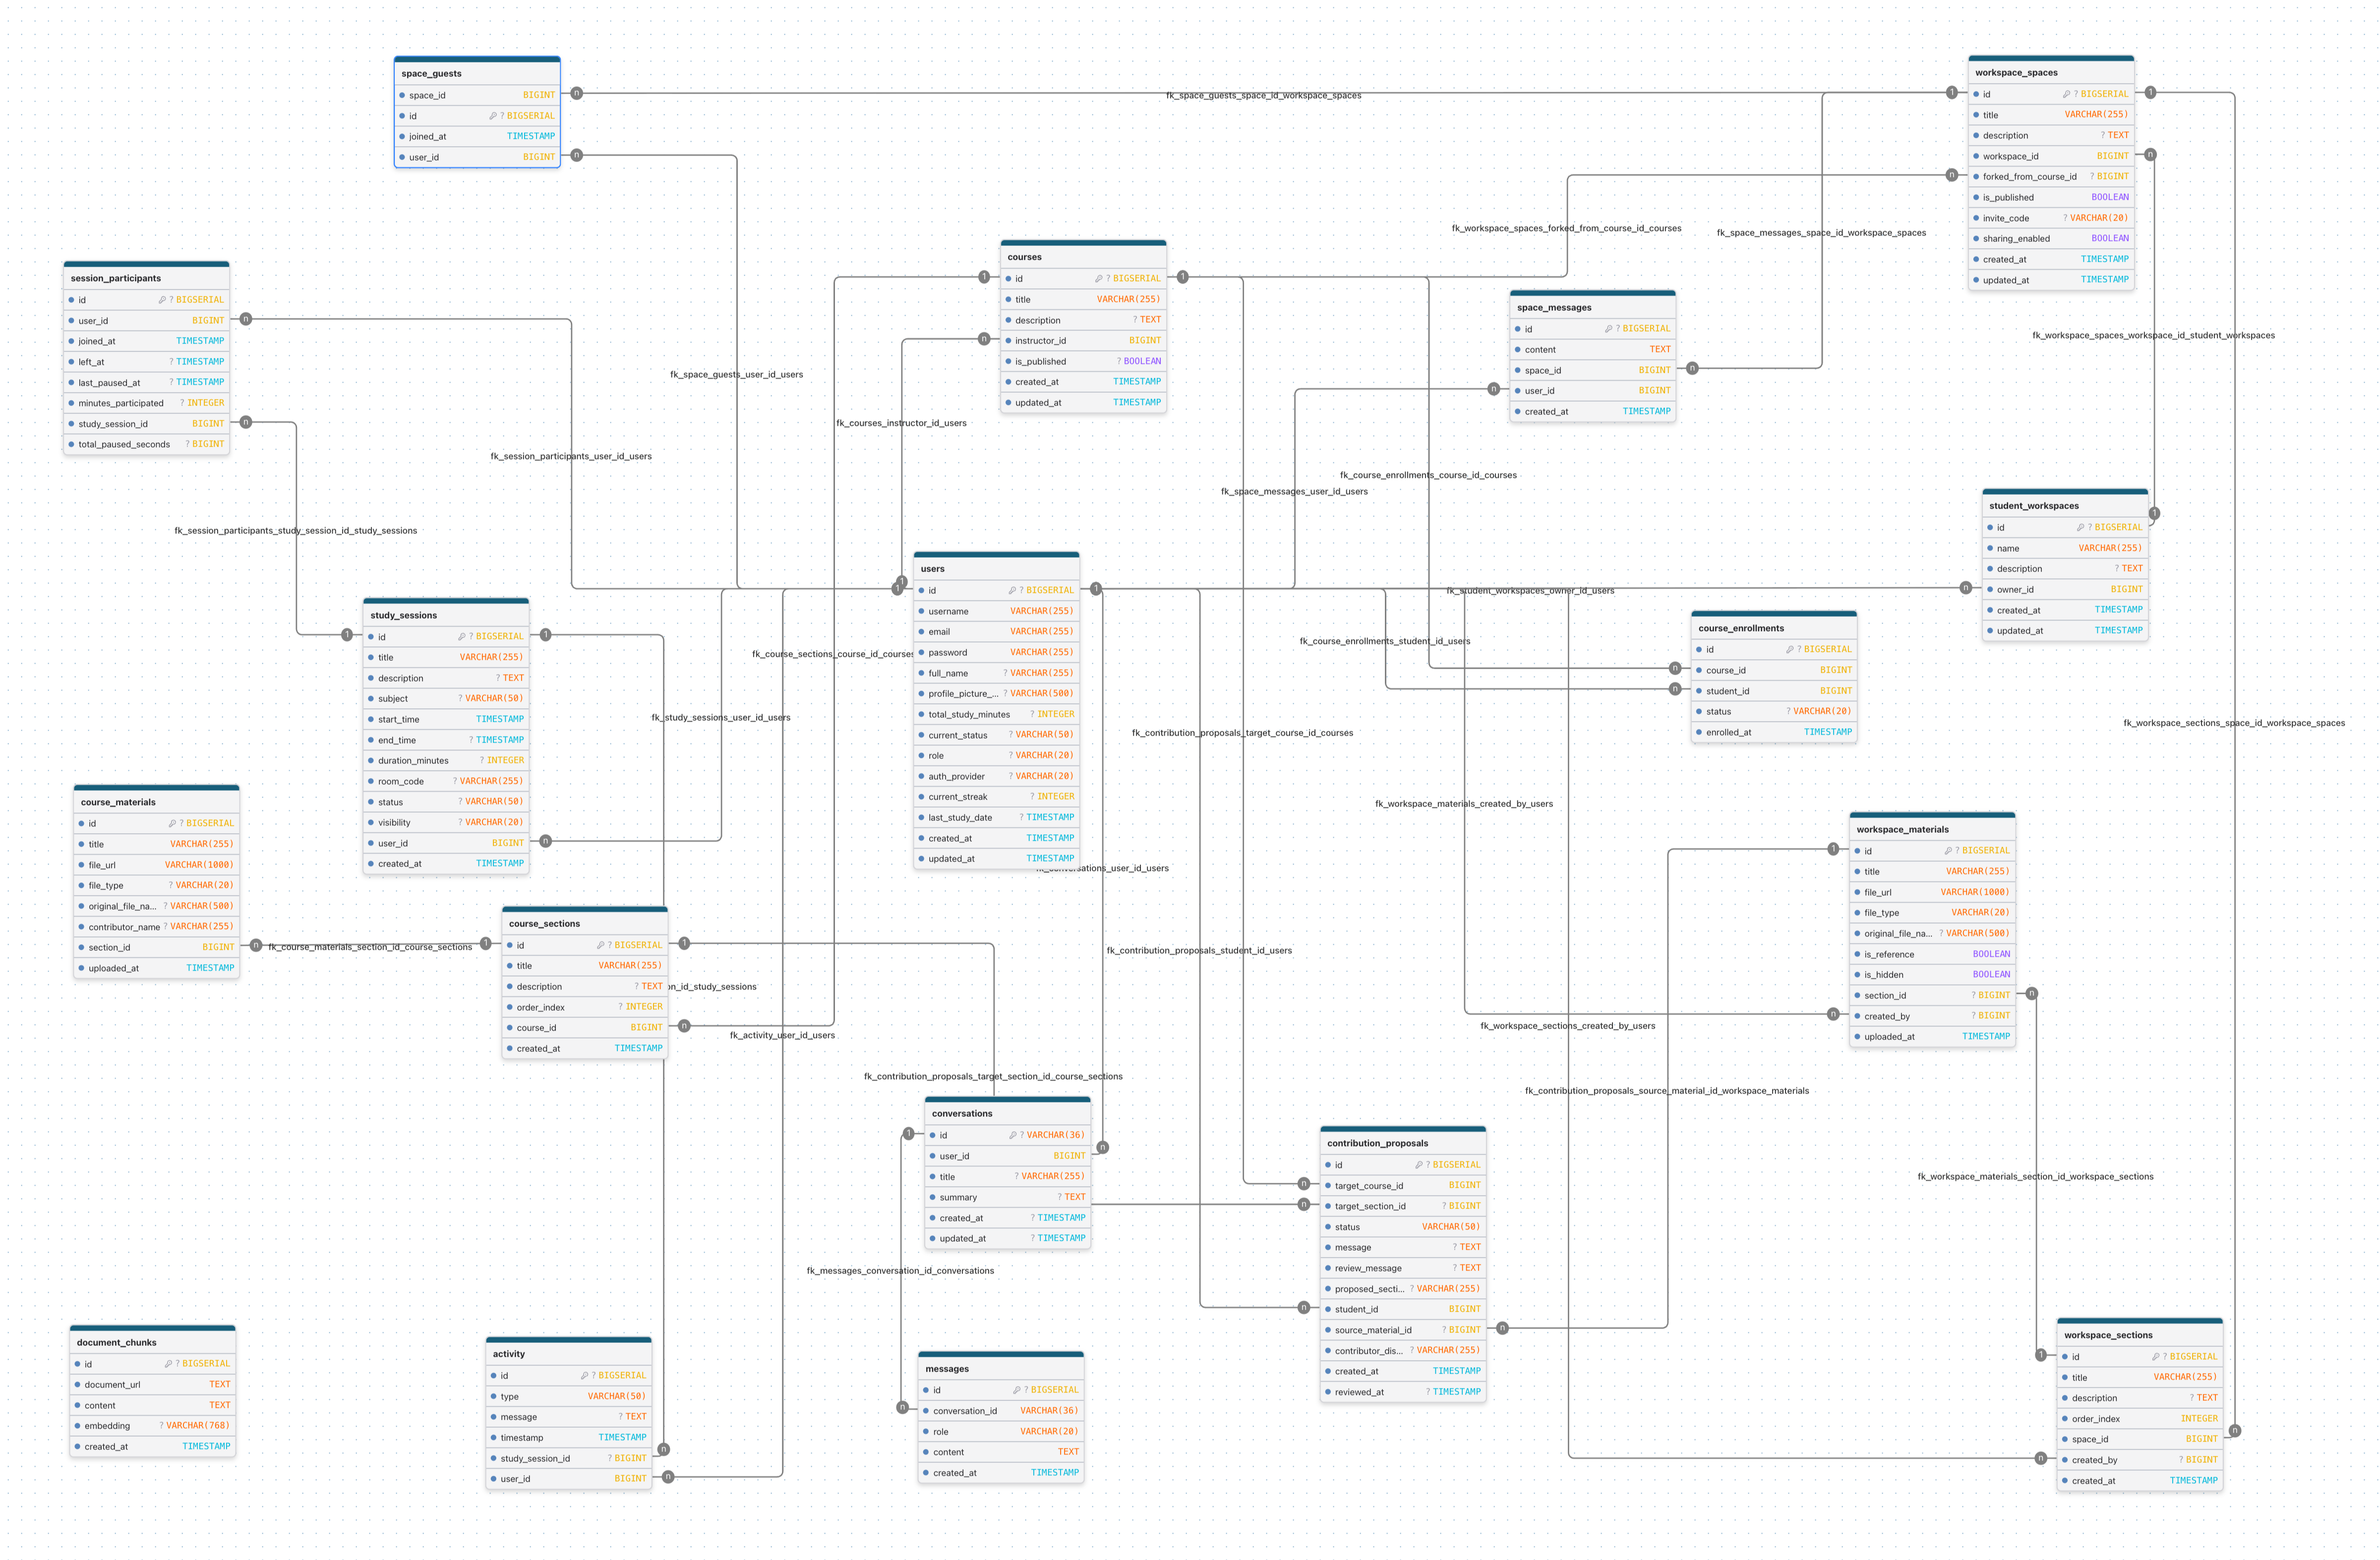
\includegraphics[width=\textwidth]{images/uml_diagrams/domain-model.png}
    \caption{Complete StudySpace domain model UML diagram}
    \label{fig:complete-domain-model}
\end{figure}
 % include `appendix.tex' from `text/' subdirectory

\backmatter % do not remove this command

\printbibliography[heading=bibintoc] % print out the BibLaTeX-generated bibliography list

\chapter{Contents of Enclosed Media}
% Contents of the attachment

	\dirtree{%
		.1 /.
		.2 README.md\DTcomment{brief description of the repository and setup instructions}.
		.2 backend\DTcomment{directory containing the backend Spring Boot application source code}.
		.2 frontend\DTcomment{directory containing the frontend Next.js application source code}.
		.2 documentation\DTcomment{directory containing the thesis documentation}.
		.3 ctufit-thesis.pdf\DTcomment{the final thesis text in PDF format}.
		.3 user-guide.pdf\DTcomment{the user guide for the application}.
		.2 docker-compose.yml\DTcomment{configuration file for running the application locally}.
	}
 % include `medium.tex' from `text/' subdirectory

\end{document}
